%!TEX root = ../main.tex

\chapter{計算例}
本章では，例題を用いて計算を行った結果を示し，本研究で作成した2つの数理モデルの妥当性や有用性について検討する.
なお，求解には最適化ソルバーとしてpySCIPOptを用いた\cite{x}．

\section{問題設定}
高知県内の某工場を対象に電力運用最適化モデルを導入し，2025 年7月3日木曜日0時00分から7月9日水曜日23時59分までの1週間についての運用計画を考えるケースを想定する．
各々の期の刻み幅$\Delta t$は1分とする．
このとき，$K = 60 \times 24 \times 7 = 10080$となる．
本例題では，工場側から「余剰電力の売電を考慮し，正味の支出を最小化したい」という要求があるものとし，
ケース2に基づいて検討を行う．

\subsection{太陽光発電設備}
1週間先までの太陽光発電量の予測値が，1分刻みの時系列データとして与えられているものとし，
これを$g_k^{\rm P1}$に代入する．
本計算例における$g_k^{\rm P1}$の値を図\ref{fig:lp_gP1}に示す．
なお，以降の折れ線グラフにおいて，赤色は決定変数，青色は従属変数，緑色は外生変数を表すものとする．
\begin{figure}[h]
	\centering
 	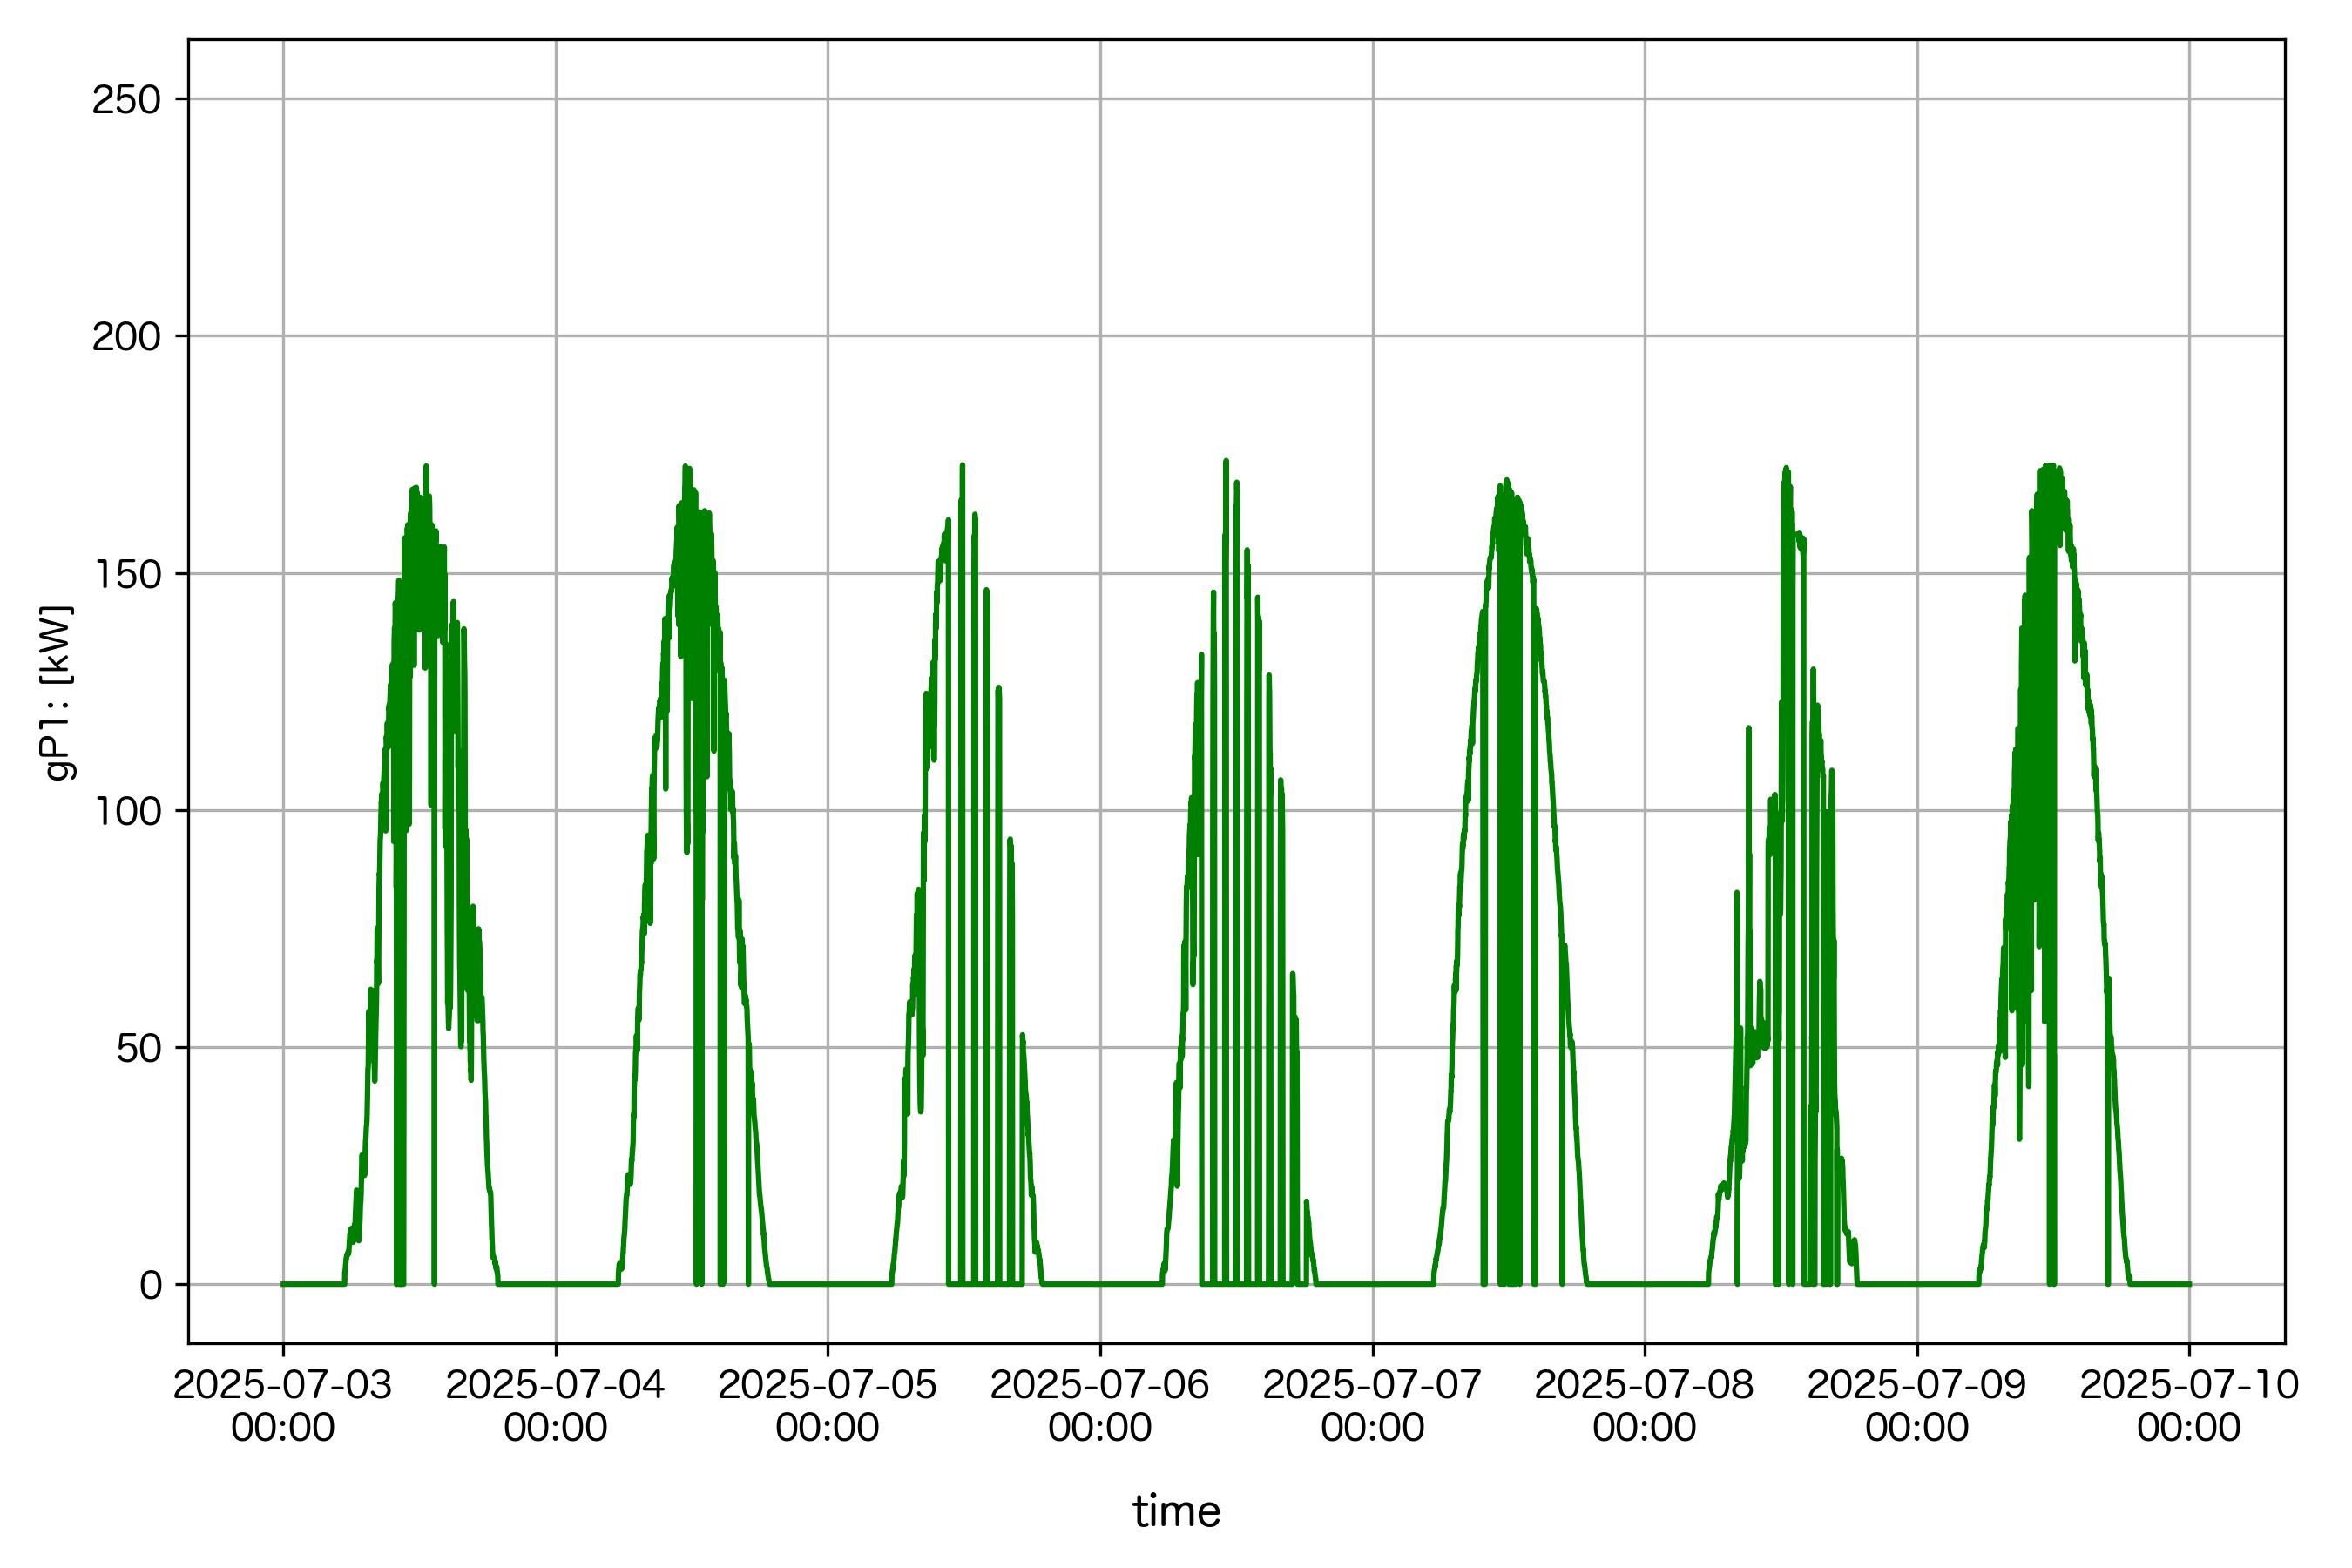
\includegraphics[width=120mm]{../figure/lp/gP1.png}
 	\caption{Solar PV Generation (Before Conversion)}
 	\label{fig:lp_gP1}
\end{figure}

\subsection{電力消費機器}
1週間先までの電力消費機器の電力消費量の予測値が，1分刻みの時系列データとして与えられているものとし，
これを$d_k^{\rm DA},d_k^{\rm DB},d_k^{\rm DC}$に代入する．
本計算例における$d_k^{\rm DA},d_k^{\rm DB},d_k^{\rm DC}$の値を図\ref{fig:lp_dA2}〜図\ref{fig:lp_dC2}に示す．
\begin{figure}[h]
	\centering
 	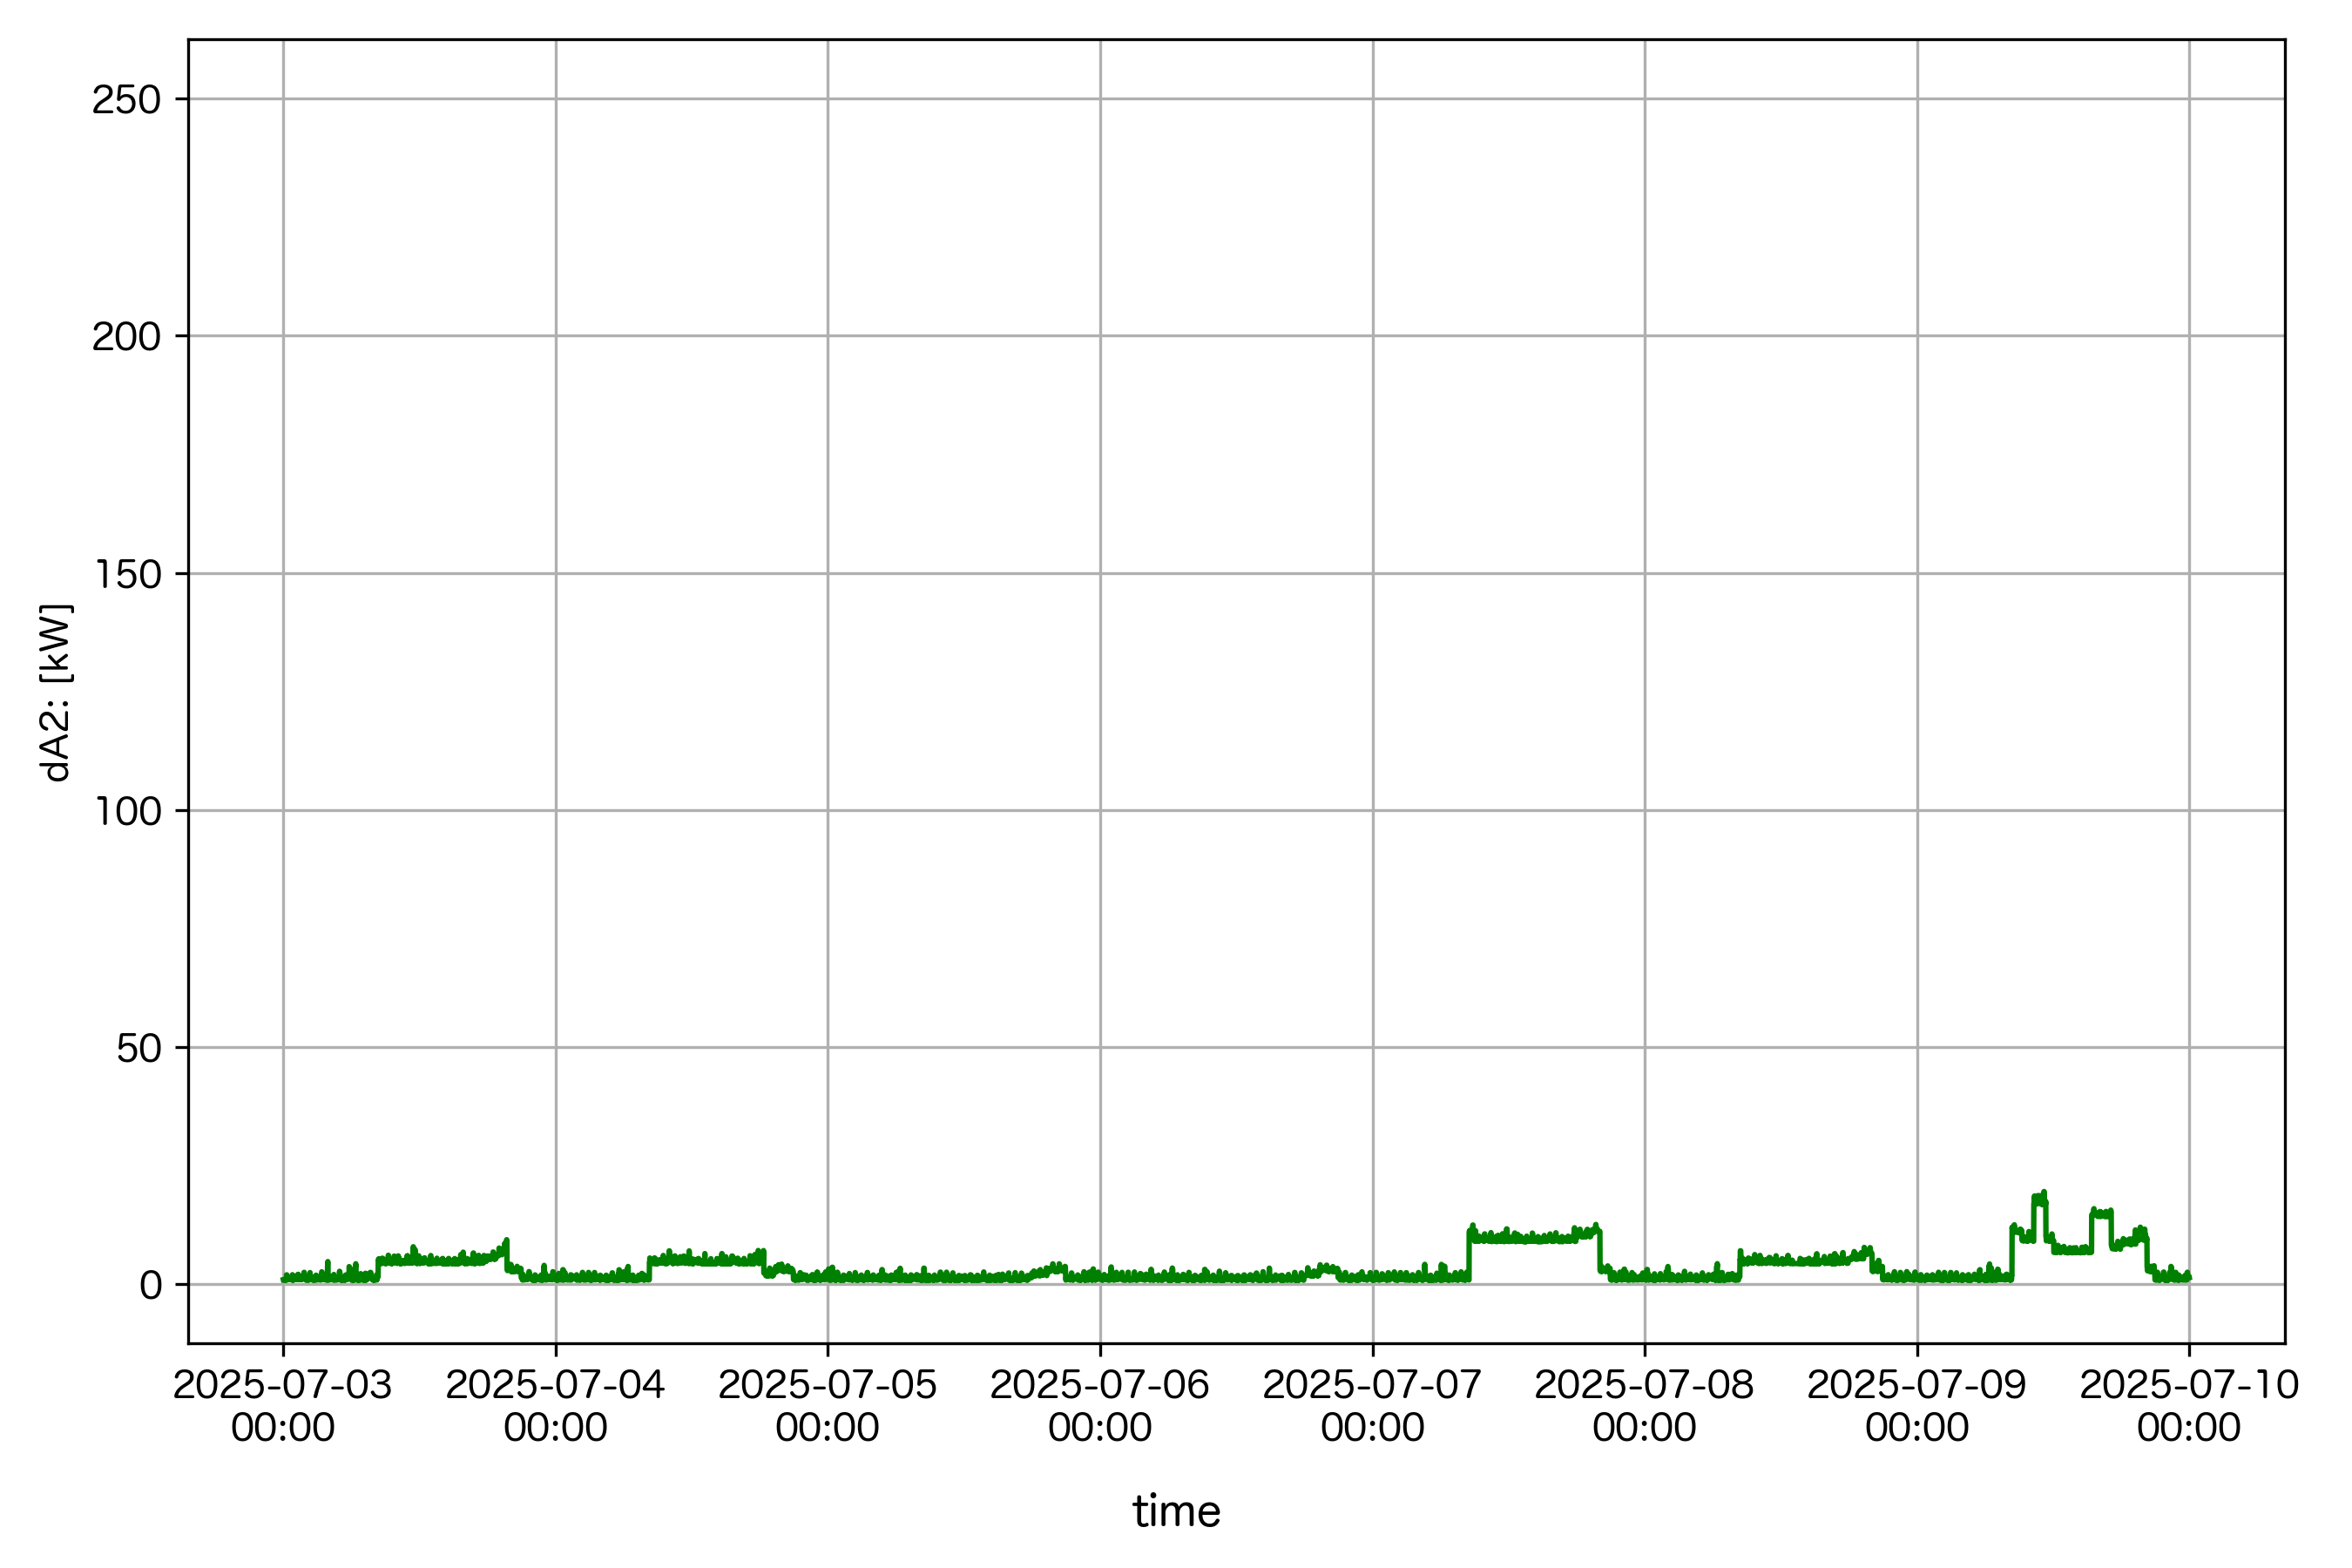
\includegraphics[width=120mm]{../figure/lp/dA2.png}
 	\caption{Power Consumption A (After Conversion)}
 	\label{fig:lp_dA2}
\end{figure}
\begin{figure}[h]
	\centering
 	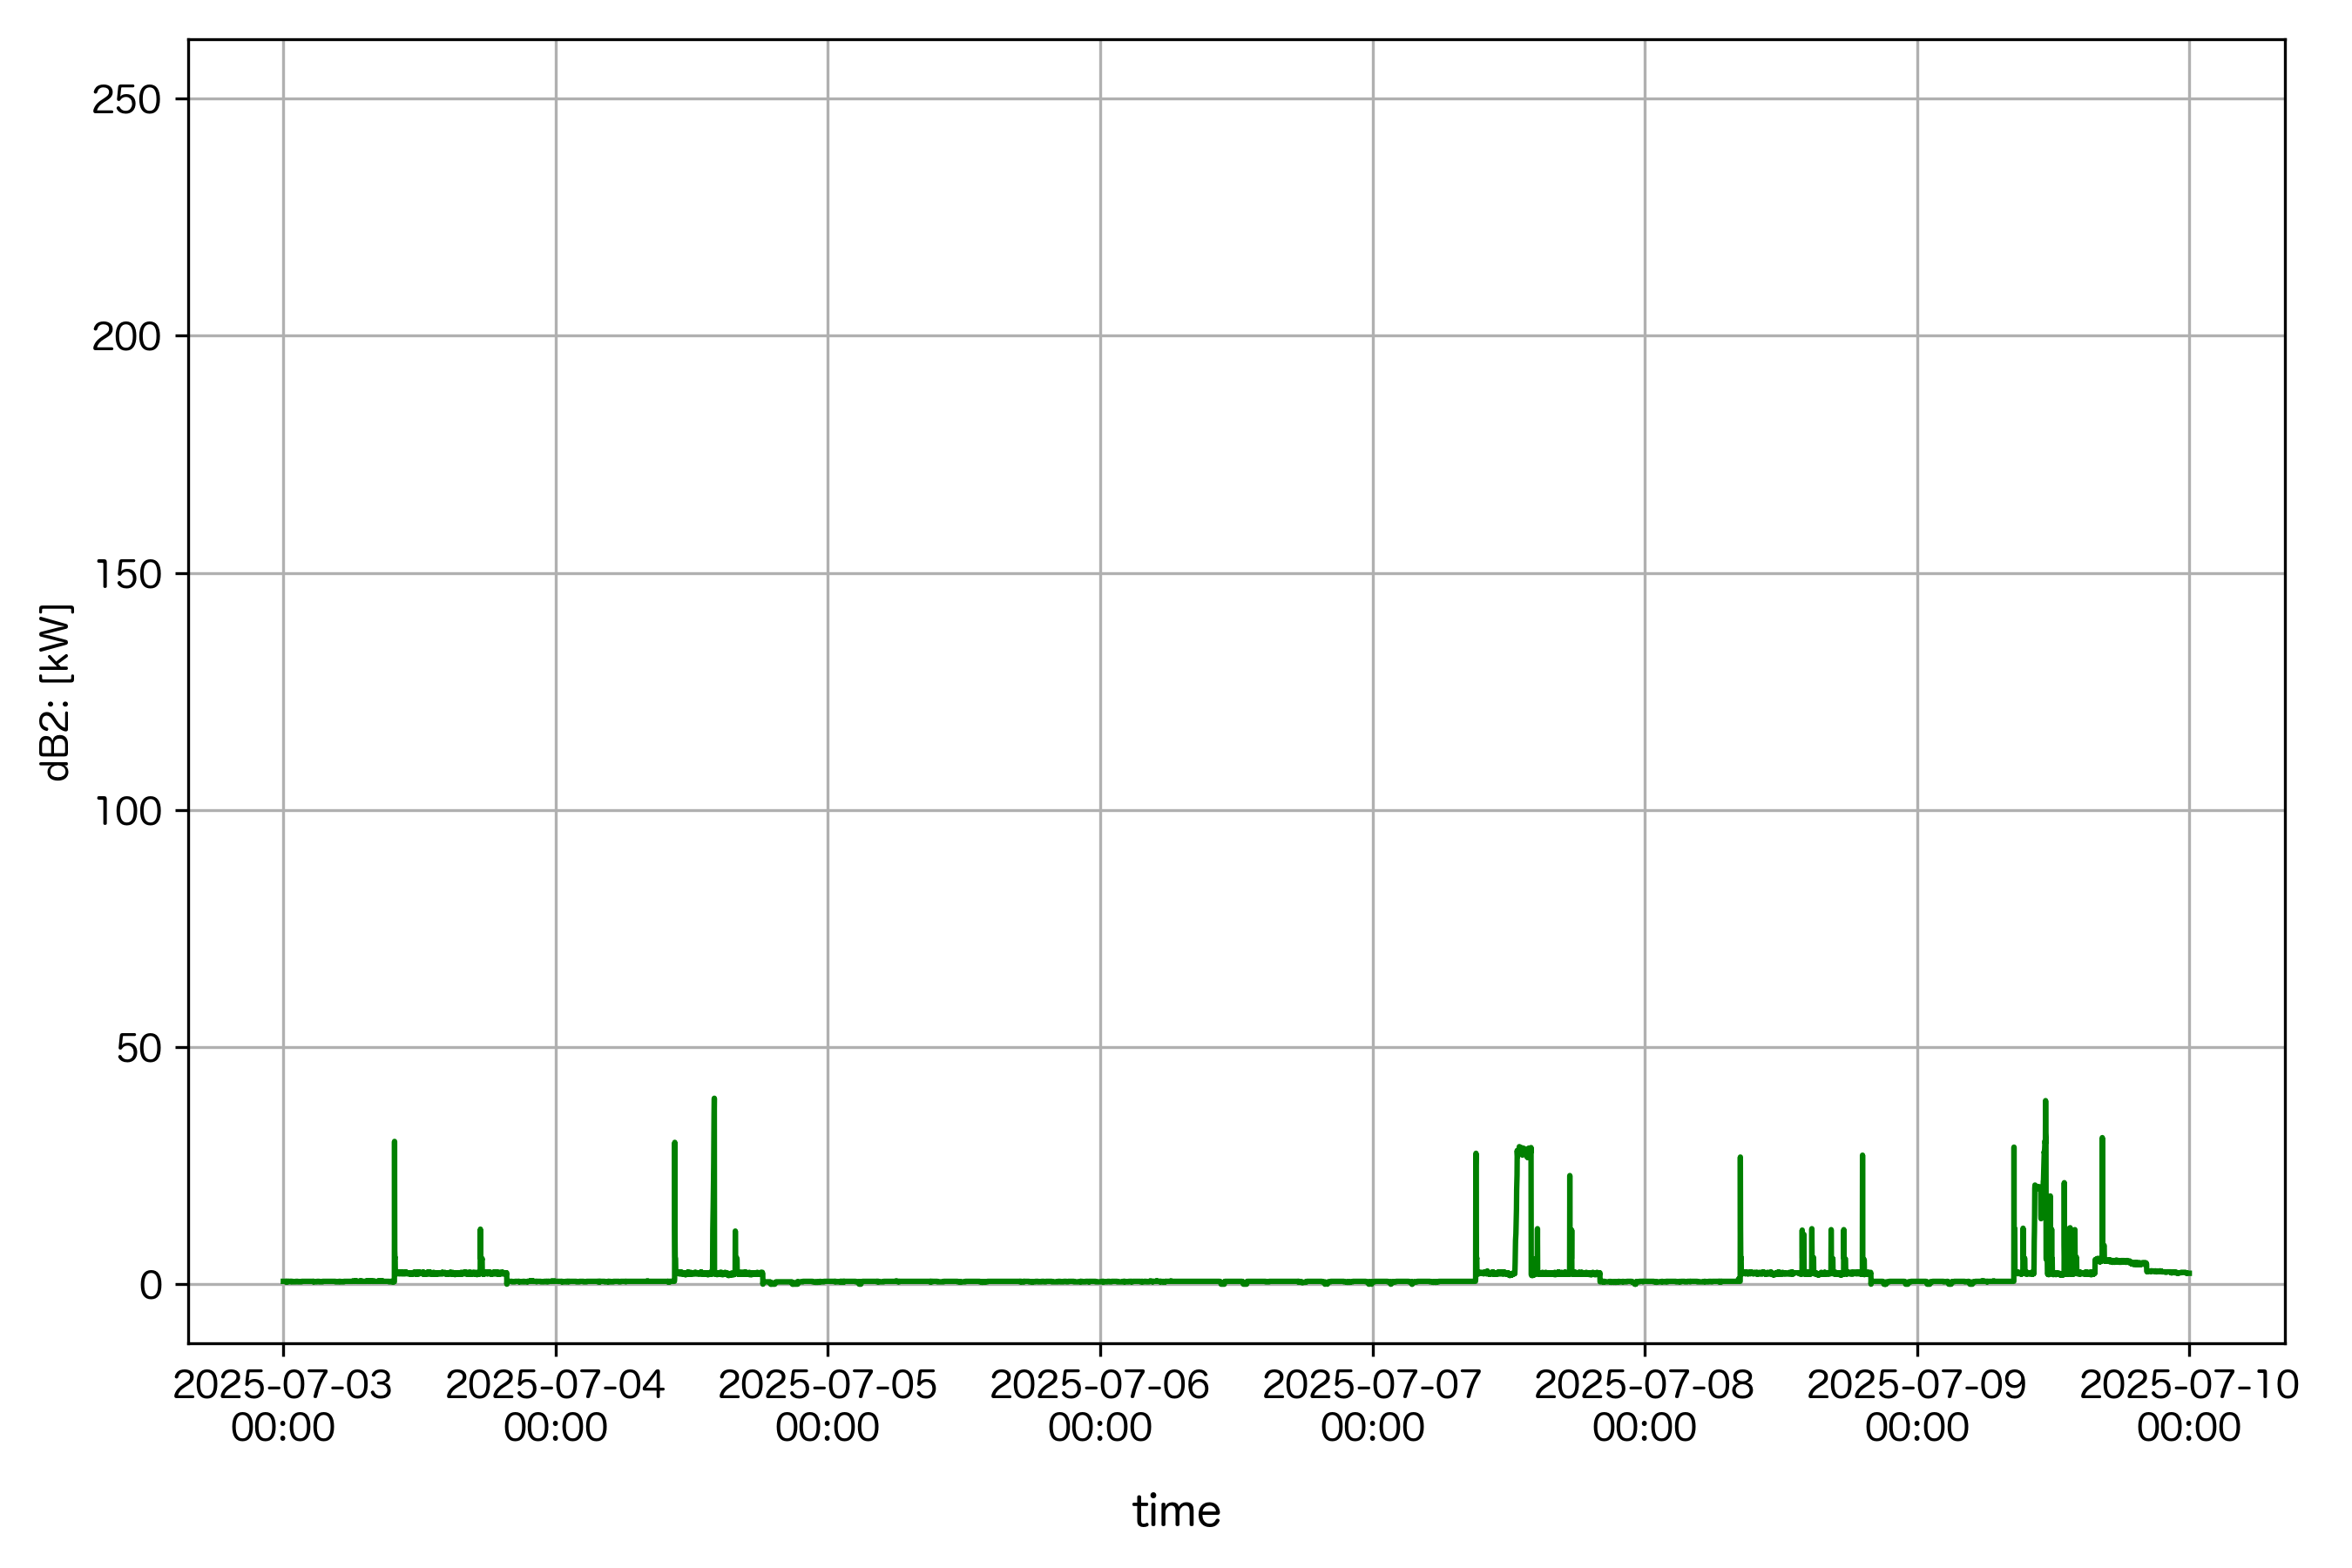
\includegraphics[width=120mm]{../figure/lp/dB2.png}
 	\caption{Power Consumption B (After Conversion)}
 	\label{fig:lp_dB2}
\end{figure}
\begin{figure}[h]
	\centering
 	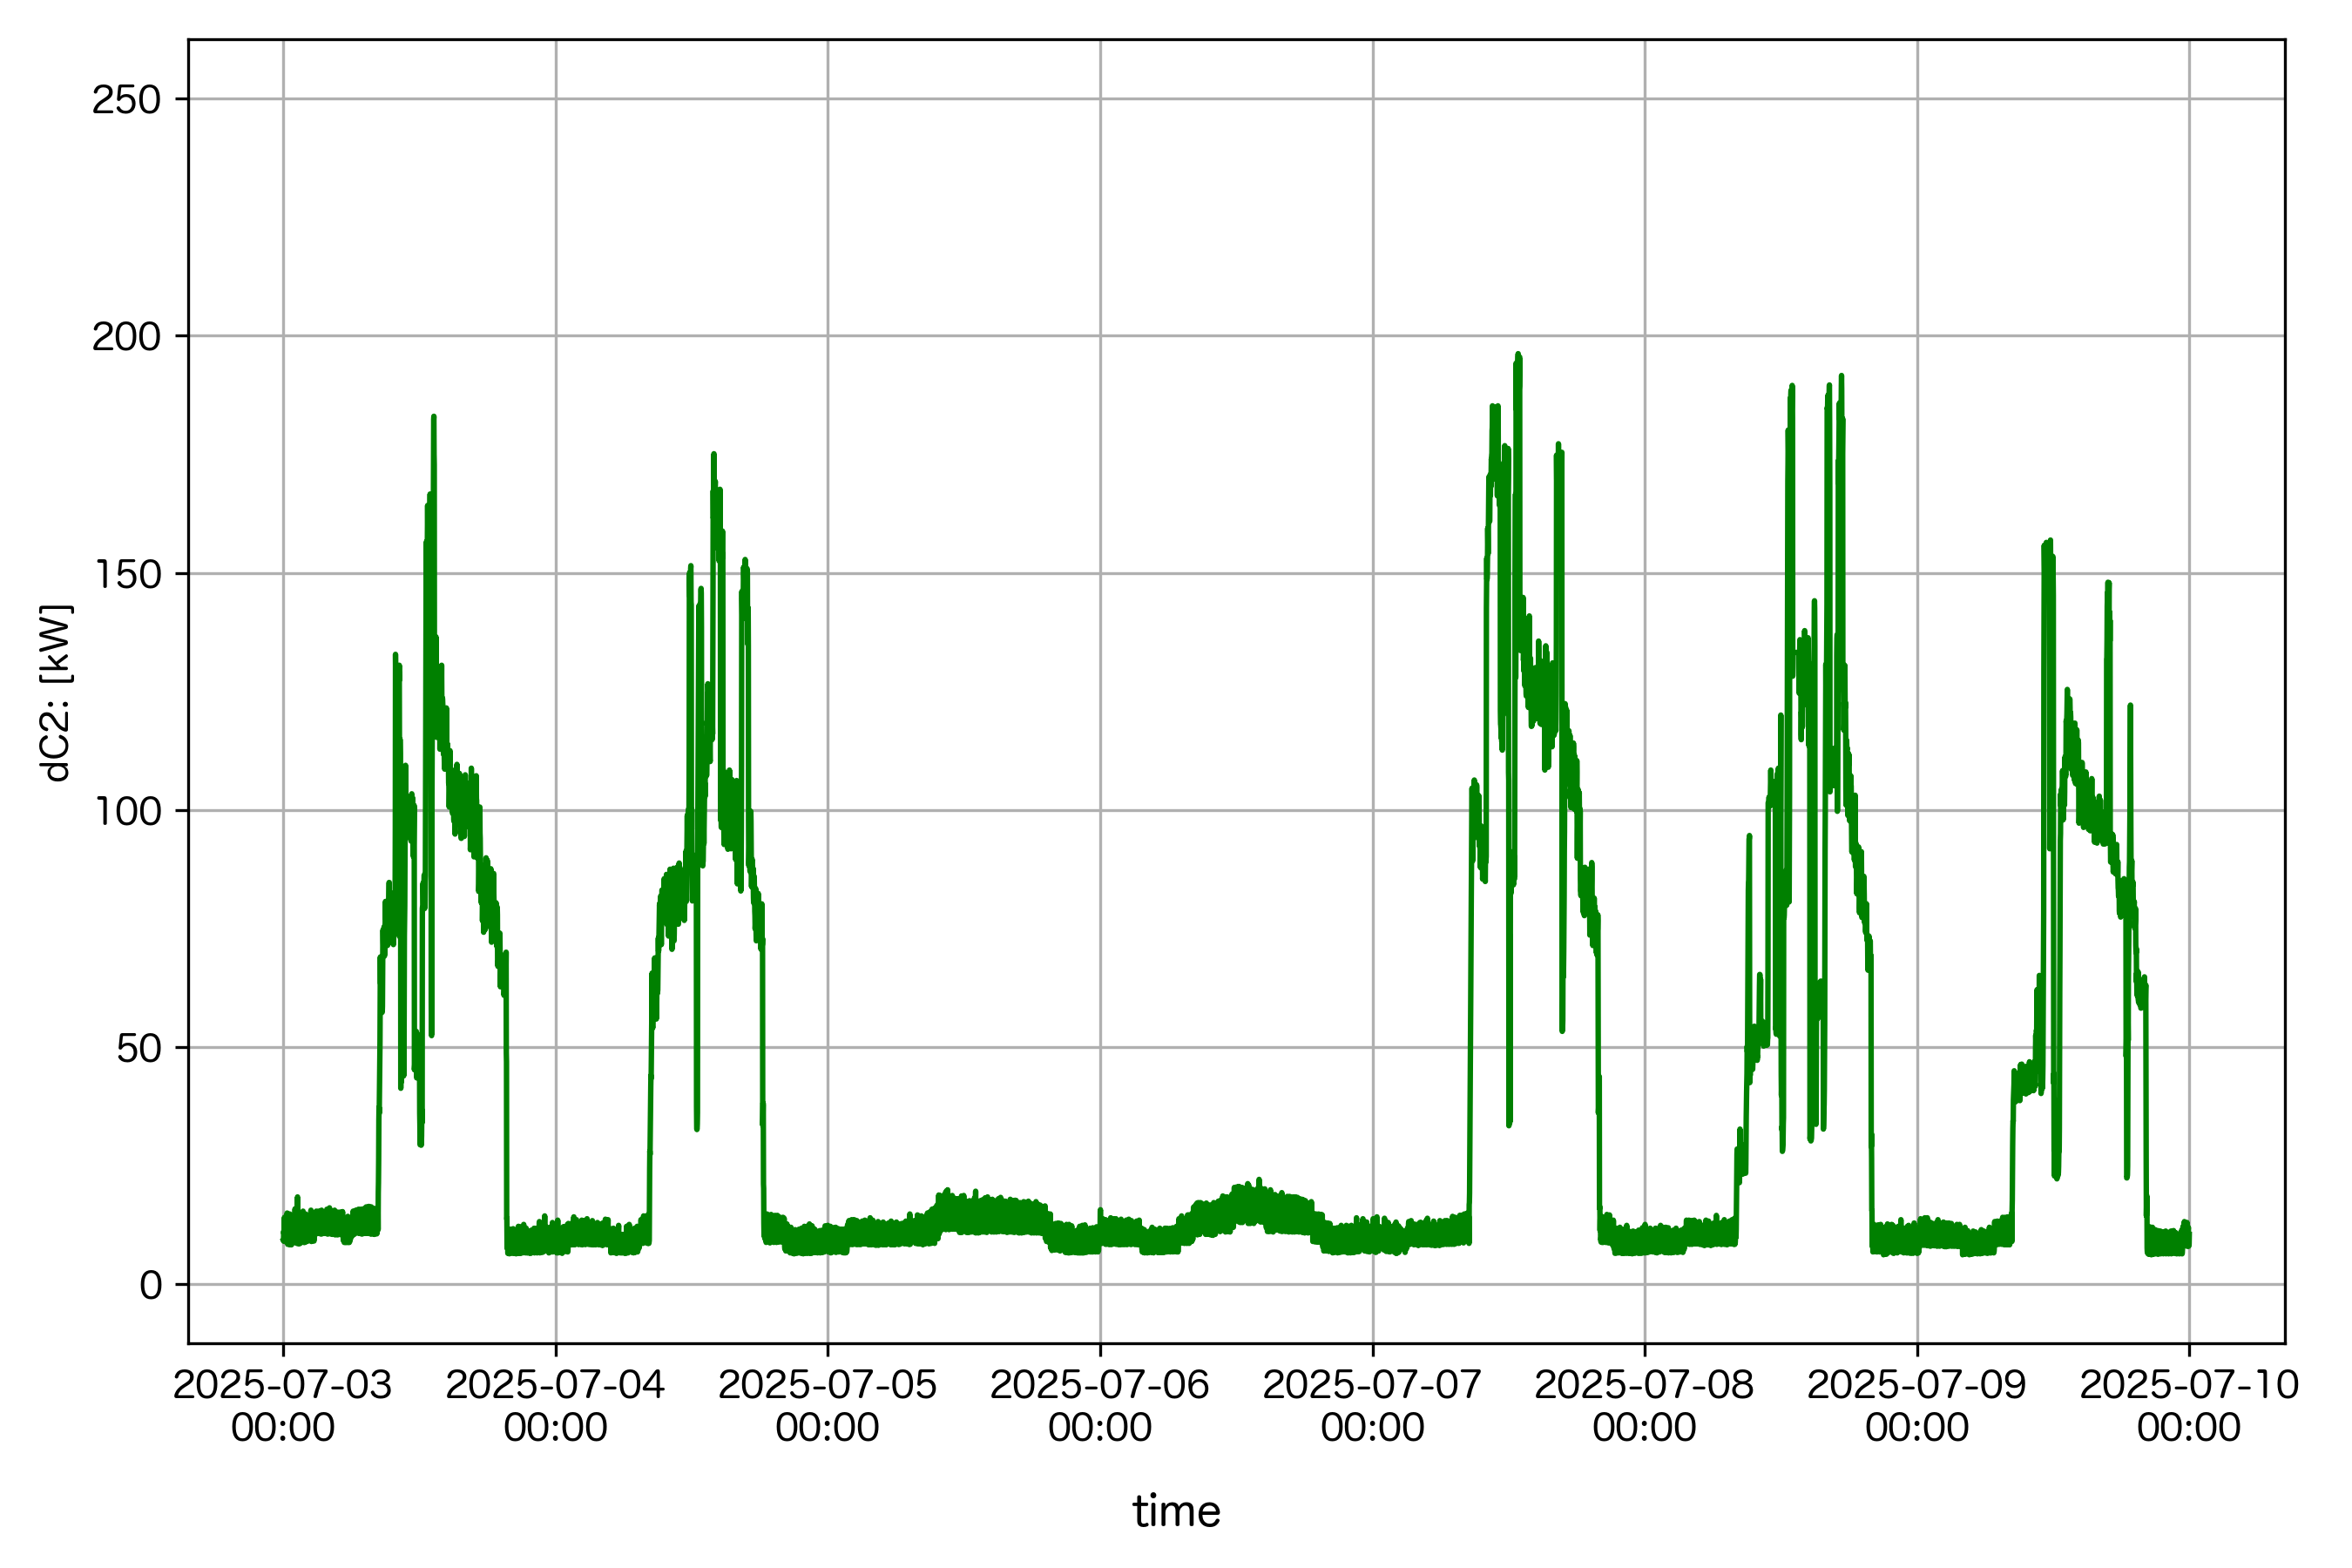
\includegraphics[width=120mm]{../figure/lp/dC2.png}
 	\caption{Power Consumption C (After Conversion)}
 	\label{fig:lp_dC2}
\end{figure}

\subsection{電力変換効率}
本研究の対象システムにおける電力変換効率を決定するため，実測データに基づく分析を行った．
図\ref{fig:efficency_g}は，電力変換器での変換前の太陽光発電量$g_k^{\rm P1}$を横軸，変換後の太陽光発電量$g_k^{\rm P2}$を縦軸にとった散布図である．

本研究では待機電力等を無視しており，変換器の物理的特性上，入力電力が0であれば出力電力も0となることから，
切片が0である一次関数で近似するのが妥当であると考えた．
最小二乗法を用いて回帰分析を行った結果，回帰直線の傾きとして$0.9449$が得られた．

本研究においては，他の電力変換器に関する詳細な入出力データが不在である．
しかしながら，一般的なパワーエレクトロニクス機器の変換効率は概ね同程度の水準にあると考えられることから，
システム全体のモデル化における代表値として上記の結果を採用し，
全ての変換効率パラメータ（$\alpha^{\rm P},\alpha^{\rm DA},\dots,\alpha^{\rm FD}$）を一律に$0.9449$と設定する．

\begin{figure}[h]
	\centering
 	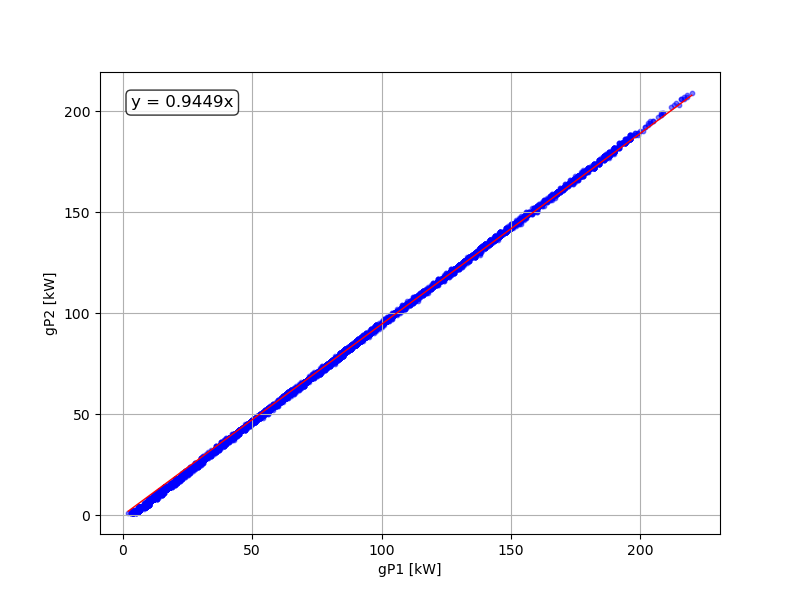
\includegraphics[width=120mm]{../figure/efficiency_g.png}
 	\caption{Correlation between input and output power in PV inverter}
 	\label{fig:efficency_g}
\end{figure}

\subsection{蓄電池}
本研究の対象に合わせ，$\overline{b}^{\rm F}$は2742 kWhとした．
なお，$b_{0}^{\rm F}$については，2025年7月3日0時00分時点における，本研究の対象の蓄電池の残量を参照し，$0.69\overline{b}^{\rm F}$ kWhとした．
また，蓄電池の最大充放電出力は450 kWであるとする．
本研究では期の刻み幅を1分としているので，$a^{\rm FC},a^{\rm FD}$は本モデルの計算ステップに合わせ$\frac{450}{60}=7.5$ kWhとした．

\subsection{商用電力系統}
1週間先までの系統電力量料金単価と系統売電単価の予測値が，1分刻みの時系列データとして与えられているものとする．
その予測値として，日本卸電力取引所（JEPX）のスポット市場における約定価格データを用いた．
JEPXの約定価格は30分単位で公開されるため，本研究では
各30分間の価格を対応する30個の期($k=30m, \dots,30m+29，m \in \{0,1,\ldots,\frac{K}{30}-1\}$）に対して一律に代入する形で入力データを作成した．
本計算例における$p_k^{\rm BY}$の値を図\ref{fig:lp_pSL}に示す．
\begin{figure}[h]
	\centering
 	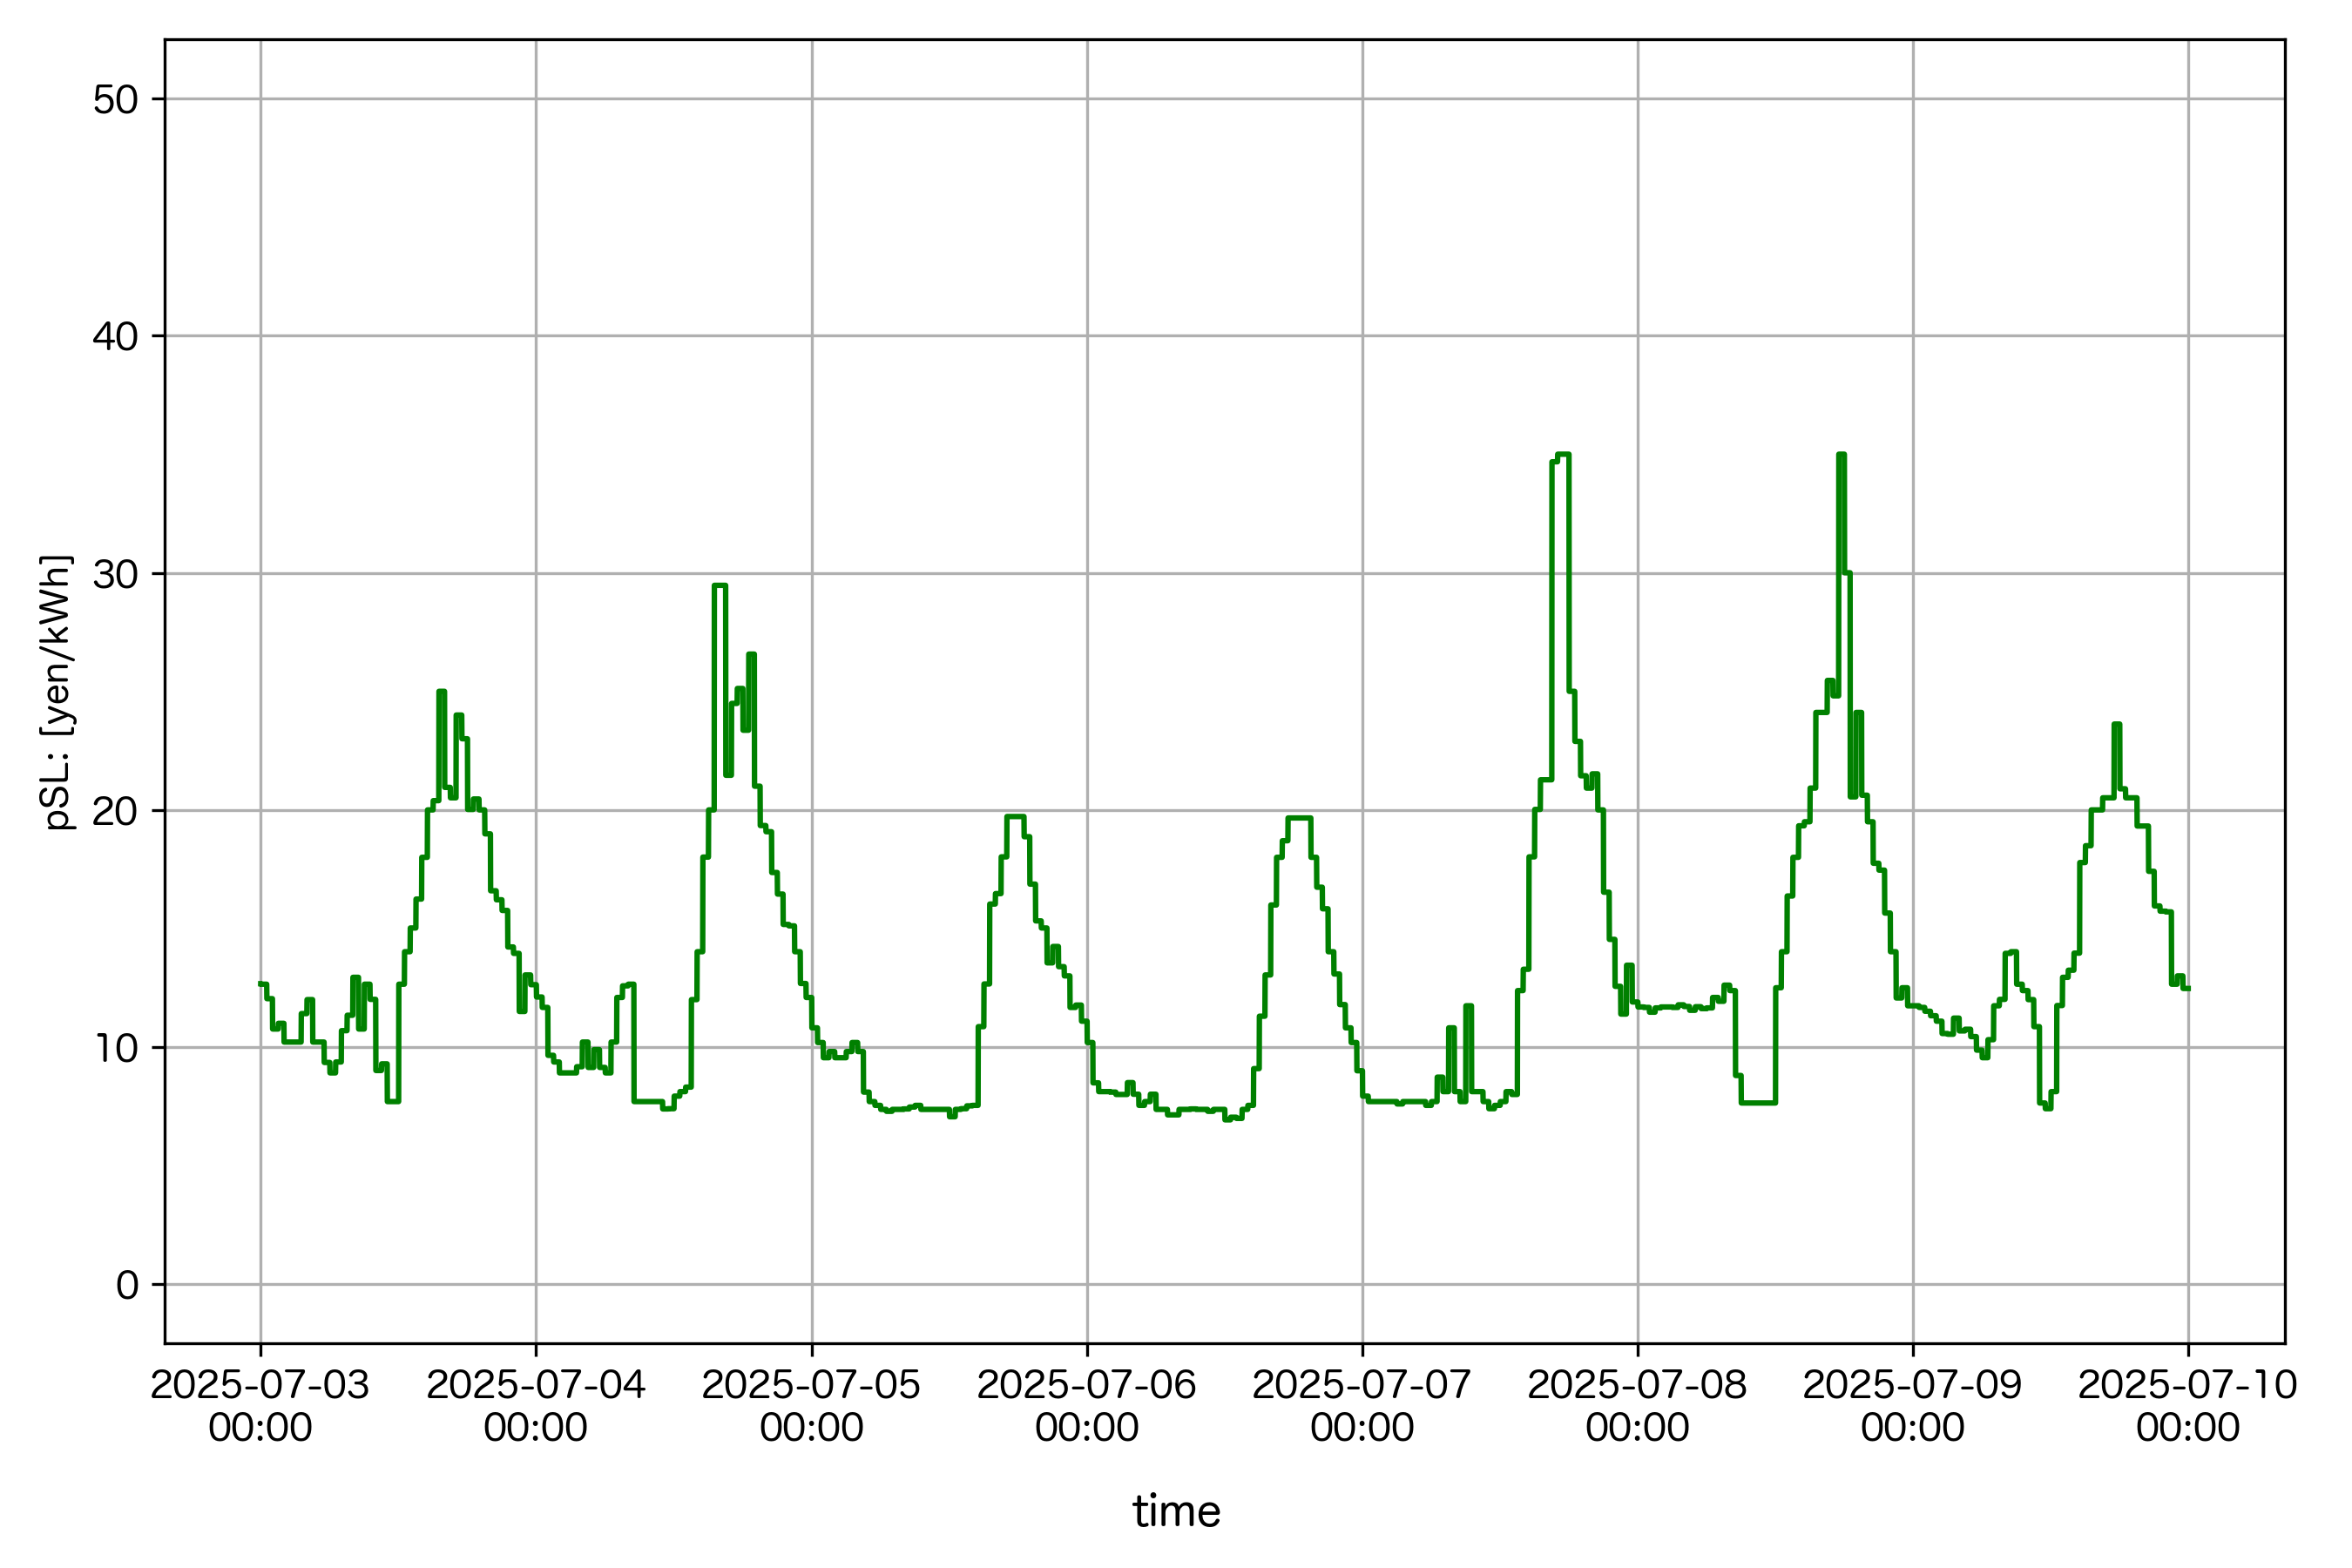
\includegraphics[width=120mm]{../figure/lp/pSL.png}
 	\caption{Electricity Purchase Unit Price}
 	\label{fig:lp_pSL}
\end{figure}

本研究で想定する市場連動型料金プランでは本来，系統買電単価と系統売電単価は同一価格となる．しかし本研究の線形計画モデルでの定式化において
$p_k^{\rm BY} = p_k^{\rm SL} $と設定した場合，同一の期に買電と売電を同時に行っても，
その収支が等しければ目的関数値に影響を与えない．その結果，最適解として同一の期に買電と売電が混在する挙動が許容される可能性がある．
このような実運用上起こり得ない現象が含まれる解を導出してしまうことを回避するために，本モデルでは系統売電単価に対して微小な負の項を導入し，
$p_k^{\rm SL}=p_k^{\rm BY} - 10^{-8}$
と定義した．こうすることにより，買電と売電を同一の期に同時に行うよりも，
いずれか一方のみを行う方が経済的に有利となる環境を数理的に構築し，同一期において買電と売電が排他的になる状態を担保することが可能となる．

また，工場からの具体的な要望として「契約電力料金の観点から，任意の連続する30分間の区間について，商用電力系統からの総買電力を 50 kW 以下に制限すること」という制約があったと仮定する．
よって，$a^{\rm BY}$は$\frac{50}{2}=25$ kWhとなる．
ところが，この制約を動的計画法の問題に反映させようとすると，
 異なる期同士が影響し合うため，過去の買電量の履歴を保持する必要があり，状態空間の増大を招くことになる．
 そのため，議論を単純にするために，この制約を元の制約より緩い制約にならないように気をつけながらより簡単な制約にしなければならない．
そこで，動的計画モデルの本計算例では「すべての期について商用電力系統から買う電力量が$\frac{50}{60}$ kWh以下でなければならない」という，期をまたがないような制約に改めた．


\section{動的計画モデルにおける，時間的計算量に関連する定数の設定}
本問題の求解にかかる時間的計算量は，更新式に則って評価値を更新する部分がボトルネックとなり，$O(B\{ \frac{(B-1)(\Delta s_k^{\mathrm{Max}}(s_{k-1}) - \Delta s_k^{\mathrm{Min}}(s_{k-1}) )}{\overline{b}} +1\} K)$となる．$\frac{\overline{b}}{B-1}$は残量の隣り合う段階の間隔であるから，
 $\frac{(B-1)(\Delta s_k^{\mathrm{Max}}(s_{k-1}) - \Delta s_k^{\mathrm{Min}}(s_{k-1}) )}{\overline{b}} +1$はある状態$s_k$について高々遷移可能な状態遷移の数を表す．
 
$K$については1週間についての運用計画を考えることが決まっていることから値を自由に変更することができない．
また，$\Delta s_k^{\mathrm{Max}}(s_{k-1})$は蓄電池の最大放電量に依存し，$\Delta s_k^{\mathrm{Min}}(s_{k-1}) $は蓄電池の最大充電量と系統からの最大買電量のうちの大きくない方に依存する値であるため，値を自由に設定することはできない．
十分高速に解を得るためには，$B$の値をどの程度の大きさに設定するのかを
考える必要がある． 

$B$に関連する制約として，「すべての期について商用電力系統から買う電力量が$\frac{50}{60}$ kWh以下でなければならない」という制約がある．
この制約をもとに$B$の値を決定することを考えるが，まず，$B$の値が小さすぎる場合，
 買電を行う状態遷移のうち，系統から買う電力量が$\frac{50}{60}$ kWh以下になるようなものが存在しなくなってしまい，
 実質的に「買電をしてはいけない」という制約になってしまう．また，残量の隣り合う段階の間隔が大きくなるため誤差が大きくなってしまうというデメリットも伴う．
 逆に，$B$の値が大きすぎる場合，遷移可能な状態遷移が多くなりすぎてしまい求解に時間を要することになる．これらを考慮して，残量の隣り合う段階の間隔が$0.2$ kWh，
 すなわち，12 kW刻みの電力となるように$B$を設定した．
蓄電池容量は$\overline{b}=2742$ kWhであるため，このとき$B$の値は13710となる．この$B$の値であれば各々の状態について，
買電を行う状態遷移が少なくとも4つ現れることになり，時間的計算量を抑えつつも，実用上十分な粒度で状態遷移を表現できる．

\section{線形計画モデルによる計算結果}
線形計画モデルでの計算結果を以下に示す．
まず，全期間の系統買電力を図\ref{fig:lp_sBY_sSL}に示す．
なお，図中の負の値は商用電力系統への売電を表している．
図\ref{fig:lp_sBY_sSL}より，7月6日を除くの6日間について，各日の午後の短い期間に集中して売電を行っていることが確認できる．
ここで，同時期の系統売電単価（図\ref{fig:lp_pSL}）を参照すると，
売電単価が高騰する期と売電の期が一致している．
このことから，本モデルは売電収益を最大化するために，単価が高い時間帯を的確に捉えた運用を実現しているといえる．

次に，全期間の系統買電力のうち特に7月3日の0時00分から11時59分までの12時間分の結果を図\ref{fig:lp_sBY_sSL_first_12h}に示す．
図\ref{fig:lp_sBY_sSL}では50 kWを超える買電が散見されるが，これは本モデルの制約が「30分間の平均電力」を対象としていることに起因すると考えられる．
具体的に図\ref{fig:lp_sBY_sSL_first_12h}を観察すると，大量に買電を行う期間と，買電を極力抑える期間が周期的に現れている．
これは，30分という時間枠の中で瞬時的に電力を購入しつつ，枠内の残りの時間で調整を行うことで，
30分平均の最大需要電力を規定値以下に抑制しようとする挙動である．
ここで，30分間の枠内では売電単価が一定であるにもかかわらず，特定の期に買電が集中している．
この要因として，式\eqref{eq:b_f}における蓄電池の自己放電が関連していると考えられる．
蓄電池は残量に比例してわずかな目減りが発生するため，モデルは損失を最小化しようと働く．
すなわち，売電を行う直前まで蓄電池の残量を低く維持し，売電の直前で集中的に買電を行うことで，蓄電期間中のエネルギー損失を抑制する運用が選択されたと考えられる．

最後に，期ごとの蓄電池残量の推移を図\ref{fig:lp_bF}に示す．図より，最終期に蓄電池の残量が0となっていることがわかる．
これは，目的関数値を最小化するために，溜まっている蓄電池の電力を全て使い切る形で売電してしまおうとしているためである．
しかし，実世界での運用は$K$期以降も連続的に継続するものである． 
したがって，実用化に際しては，翌期以降の電力需要を考慮し，期間終了時の蓄電残量に一定の下限値を設けるなどの対応が必要であると考えられる．
\begin{figure}[h]
	\centering
 	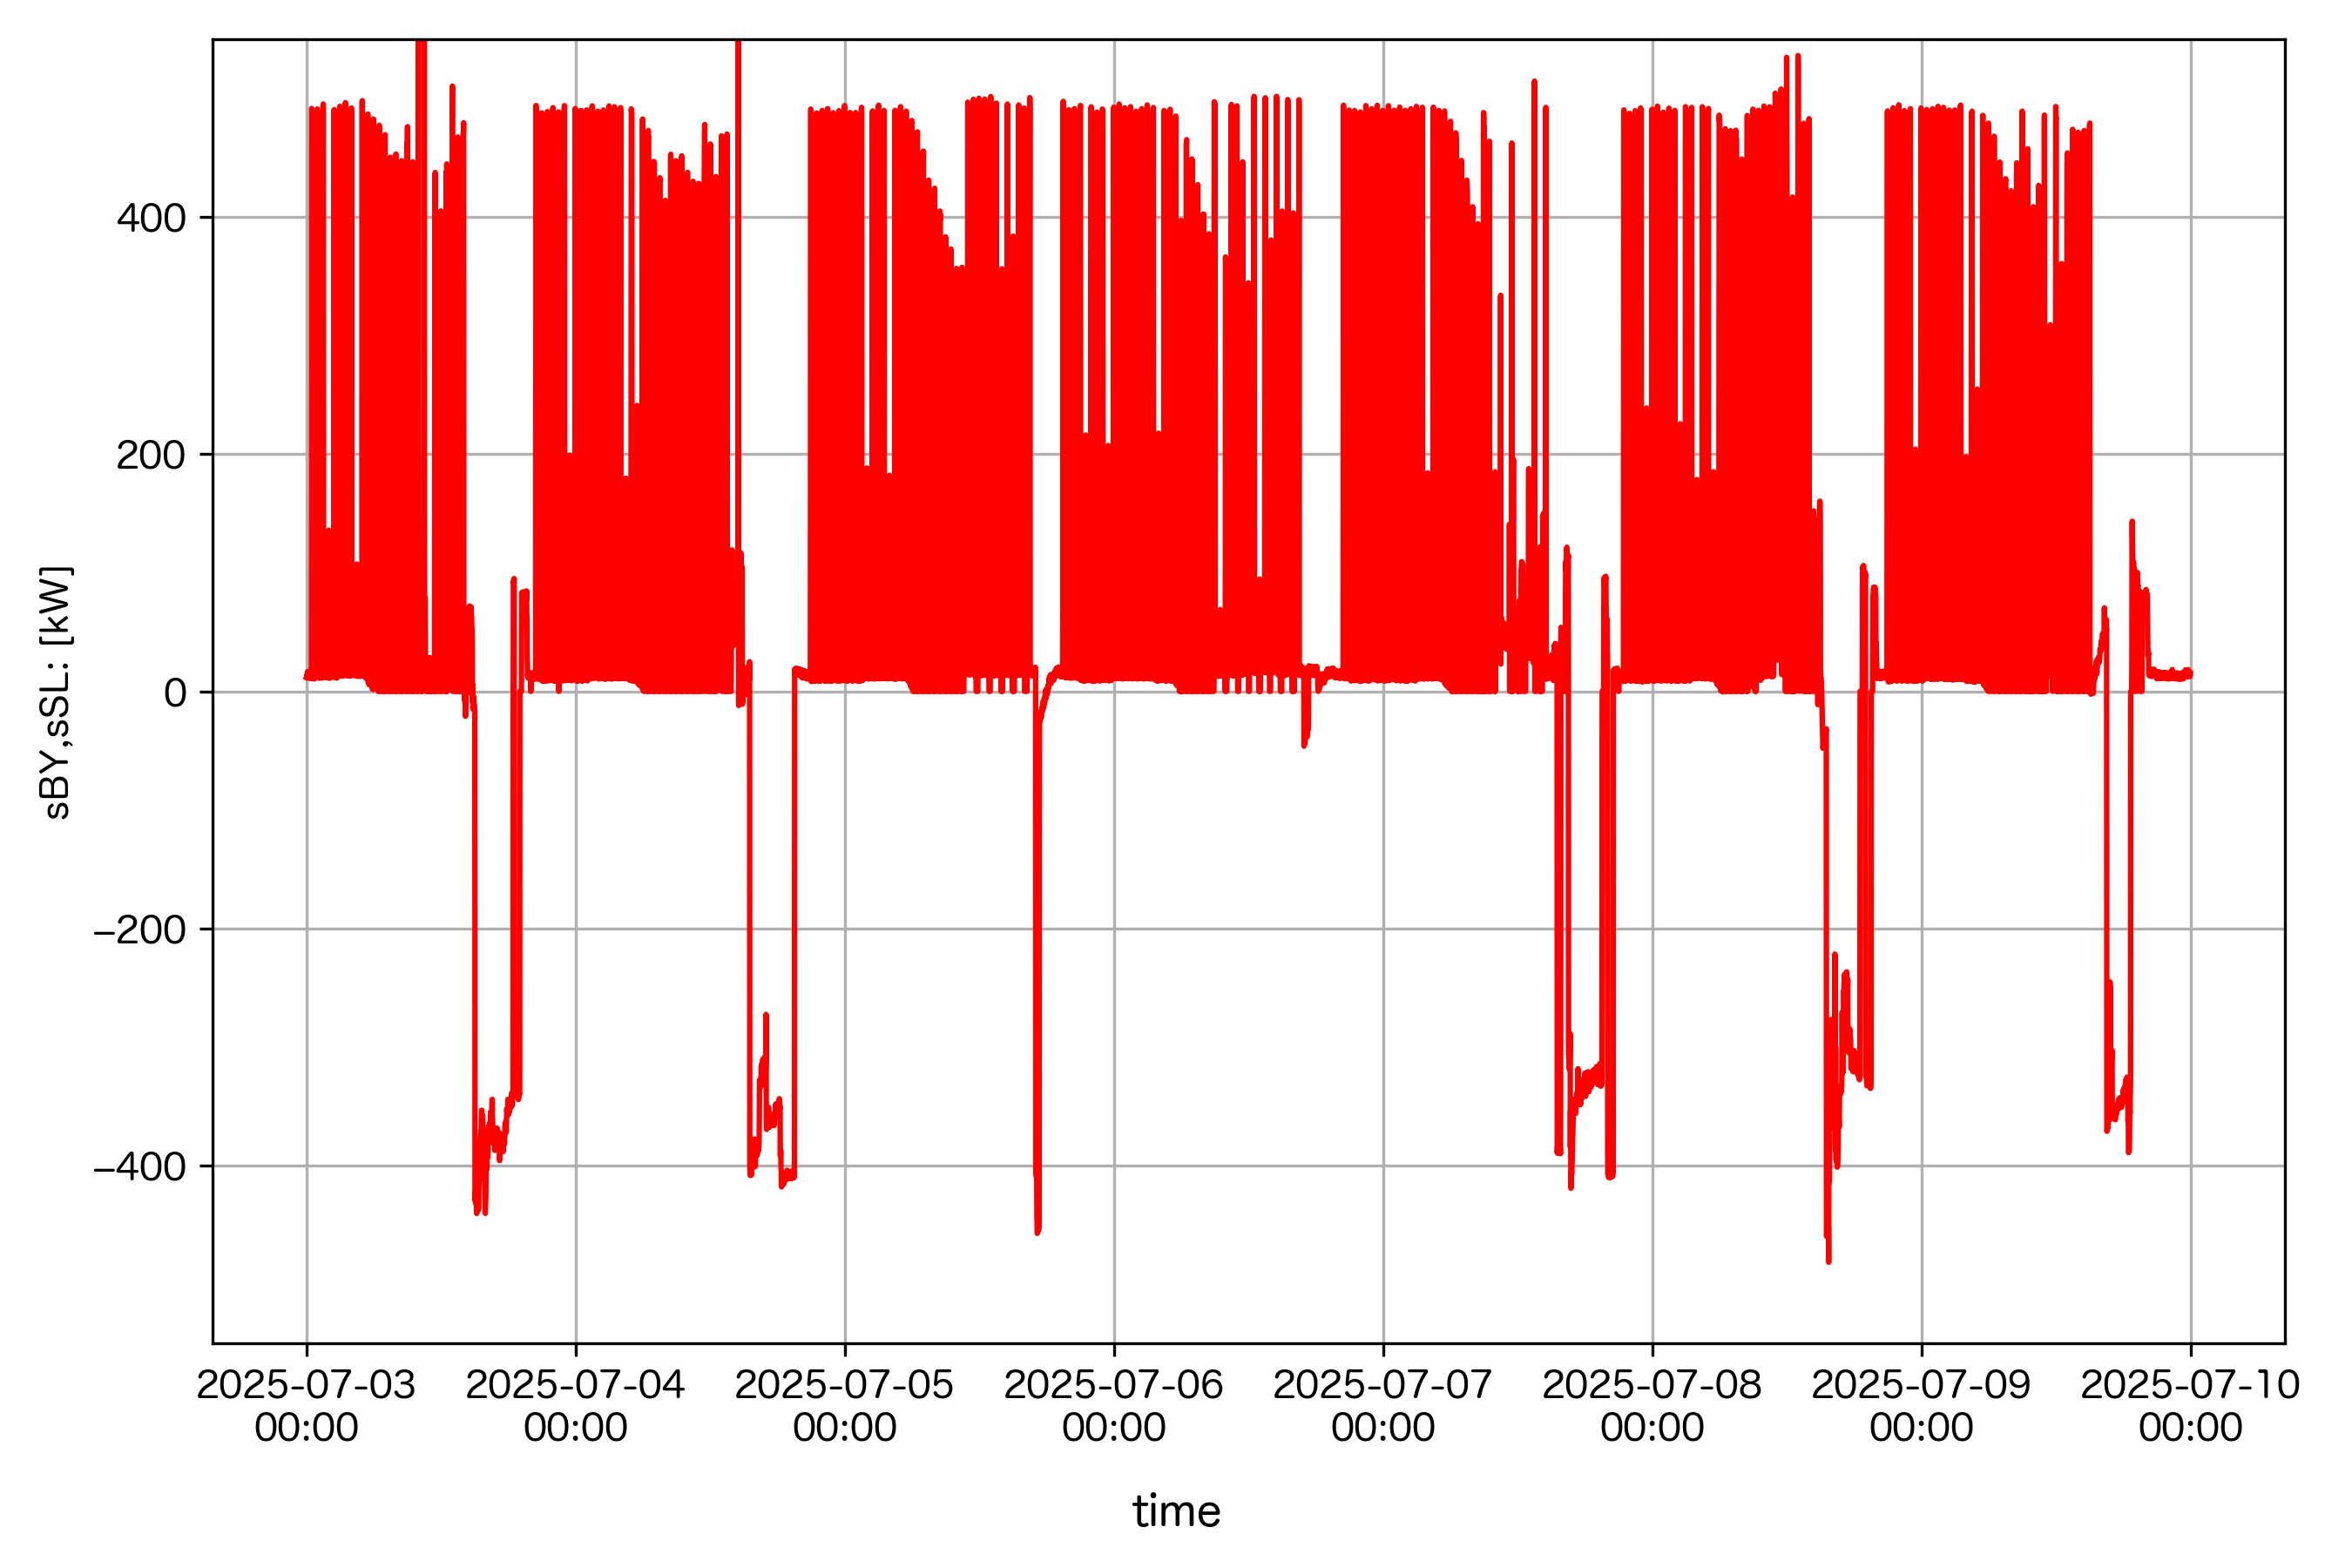
\includegraphics[width=120mm]{../figure/lp/sBY_sSL.png}
 	\caption{Grid Power Purchase}
 	\label{fig:lp_sBY_sSL}
\end{figure}

\begin{figure}[h]
	\centering
 	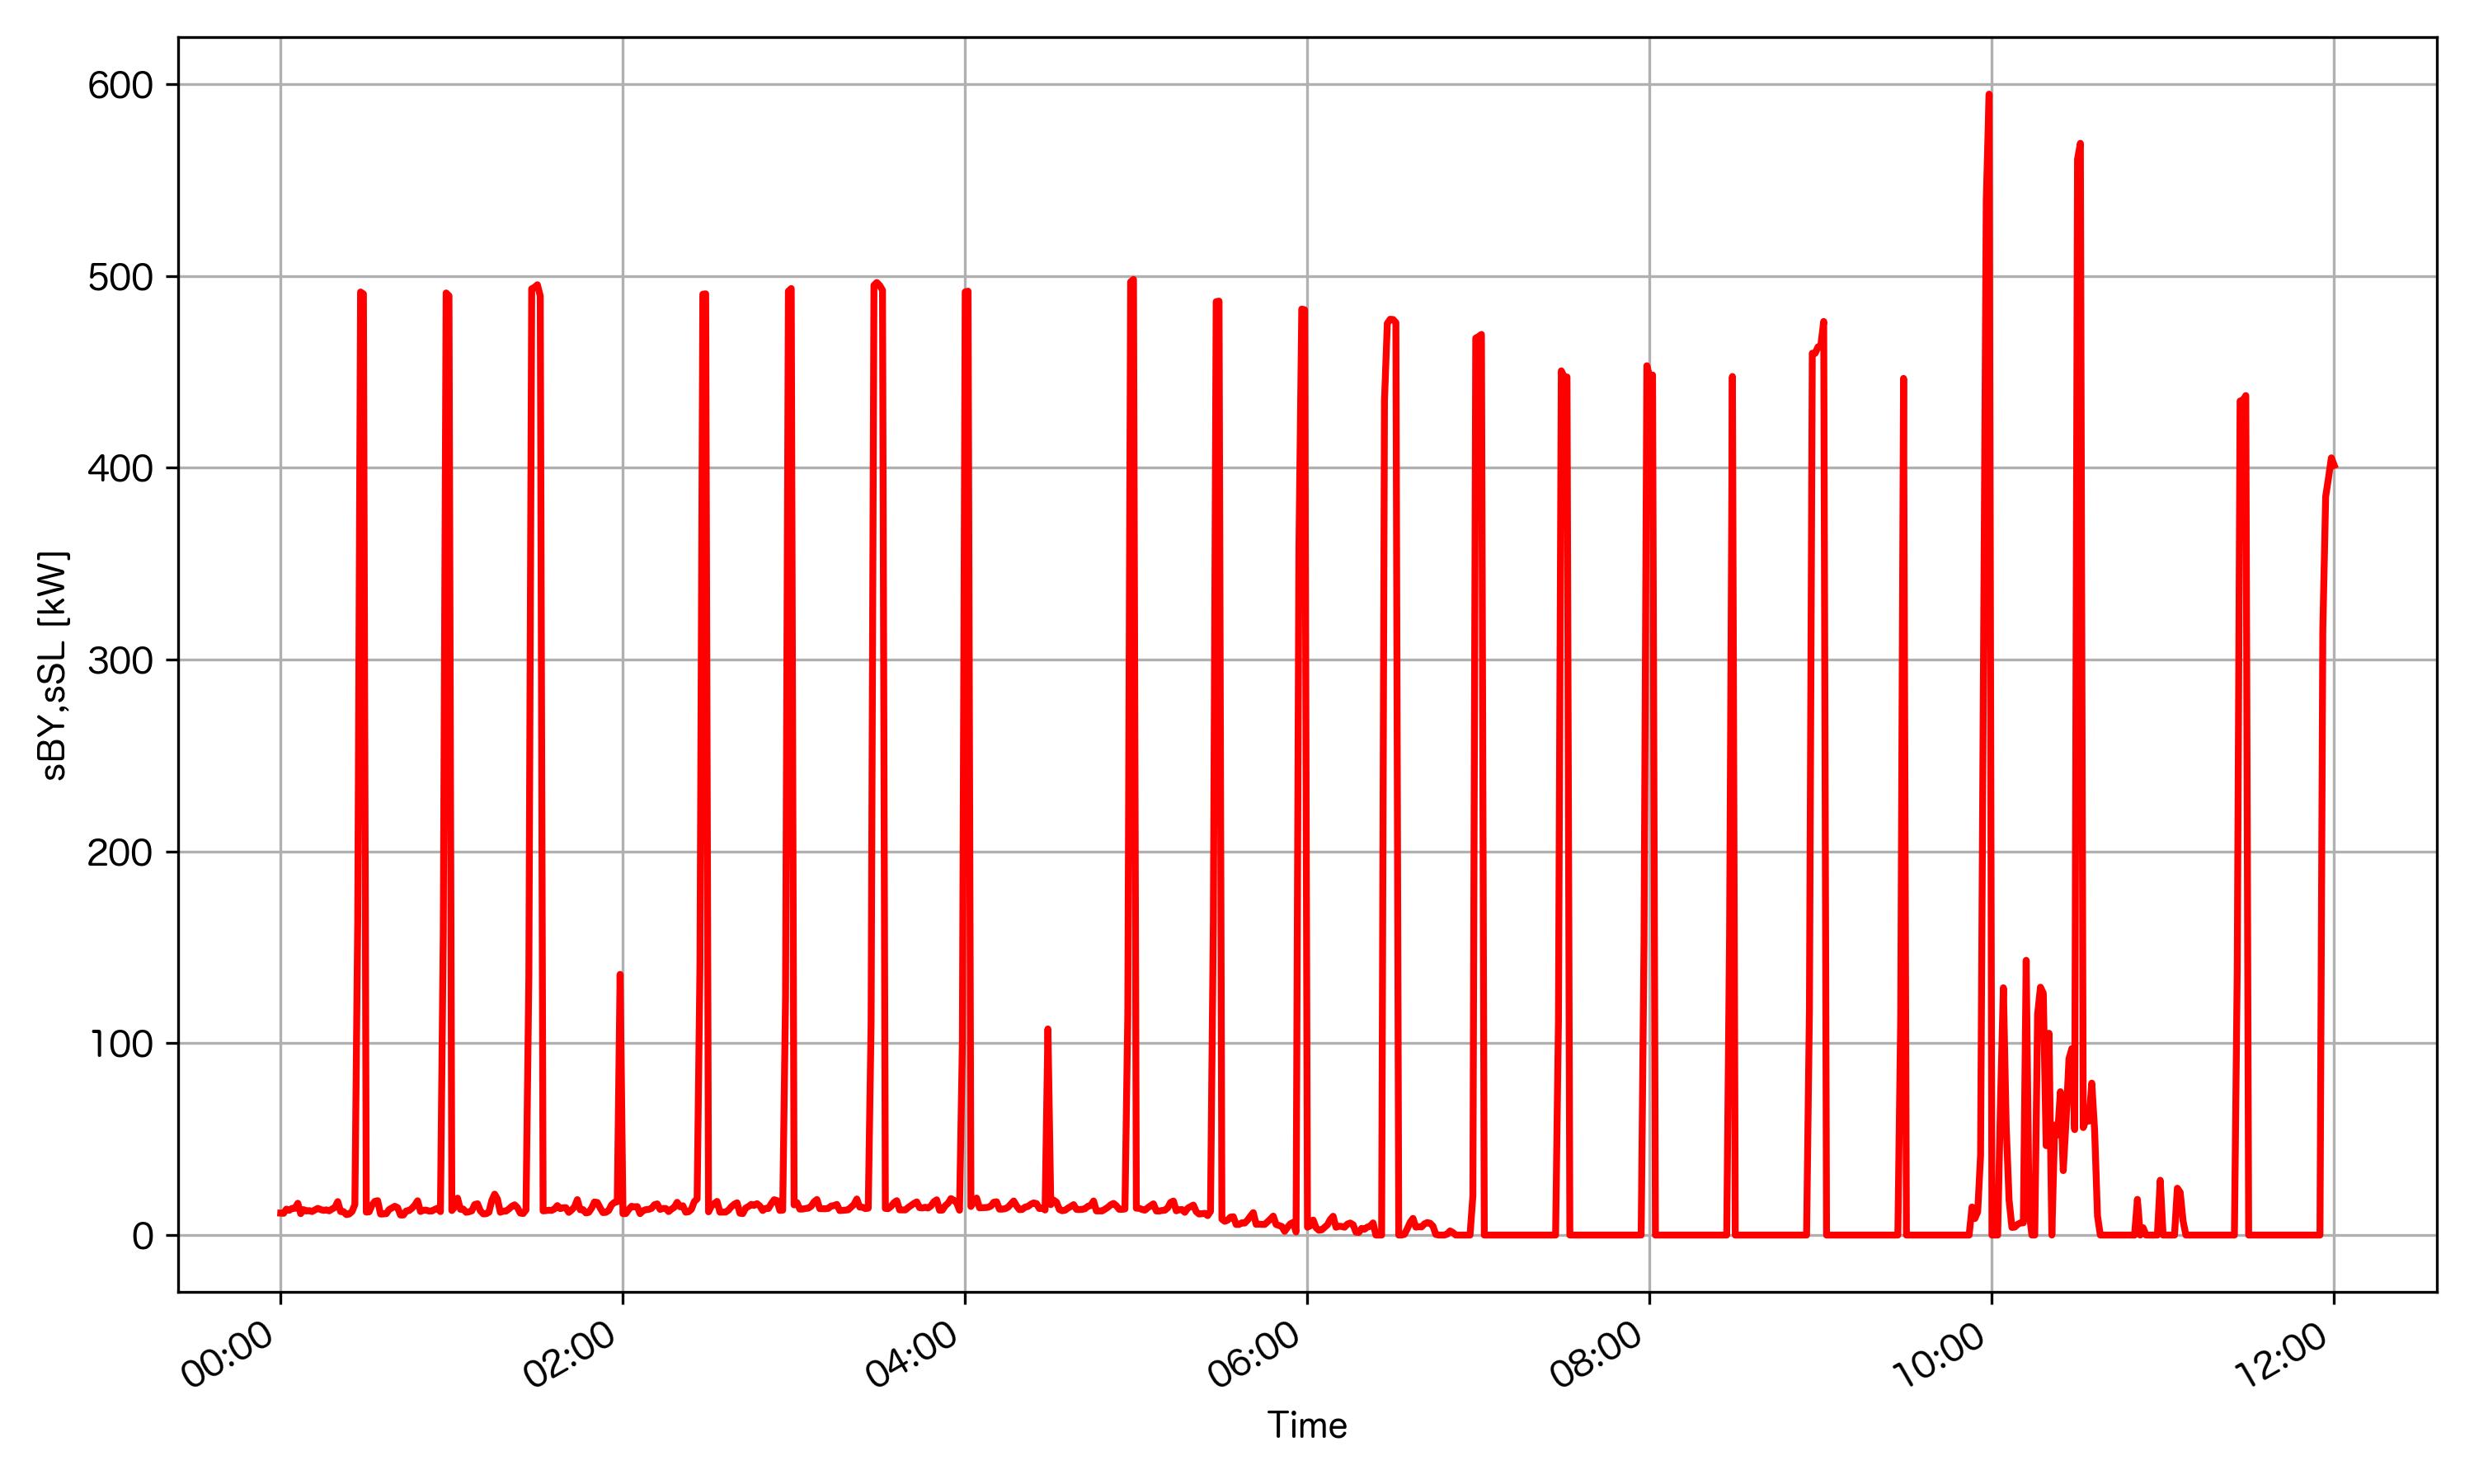
\includegraphics[width=120mm]{../figure/lp/sBY_sSL_first_12h.png}
 	\caption{Grid Power Purchase(First 12 Hours)}
 	\label{fig:lp_sBY_sSL_first_12h}
\end{figure}

\begin{figure}[h]
	\centering
 	
\includegraphics[width=120mm]{../figure/lp/bF.png}
 	\caption{Battery State of Charge}
 	\label{fig:lp_bF}
\end{figure}

\section{動的計画モデルによる計算結果}
同様の問題を動的計画モデルで解いたものを図\ref{fig:dp_sBY_sSL}，\ref{fig:dp_bF}に示す．
計算結果を確認すると，線形計画モデルと同様の期で，瞬間的に売電を行っており，
最終期の末に蓄電池の容量を使い果たすように蓄電池の電力を使用していることがわかる．
また，線形計画モデルとの顕著な相違点として，系統からの買電量が50 kWを超えている期が存在しない点が挙げられる．
線形計画モデルでは「任意の連続する30分間の区間について，商用電力系統からの総買電力を 50 kW 以下に制限すること」という制約を採用しているため，
 30分枠内で瞬間的に50 kWを超過する挙動が許容されていた．
一方，動的計画モデルにおいて同様の制約を課すためには，過去の買電量の履歴を保持する必要があり，状態空間の増大を招く．
そのため本モデルでは，状態空間の次元を抑えるために，本来30分間での制約であるものを，
1分あたりの買電力量が $\frac{50}{60}$ kWh以下であるという，より厳しい制約に置き換えて適用している．
図\ref{fig:dp_sBY_sSL}において買電量のピークが低く抑えられているのは，この制約条件の違いによるものである．
しかしながら，図\ref{fig:dp_bF}に示す蓄電池残量の推移は線形計画モデルの結果と概ね一致している．

\begin{figure}[h]
	\centering
 	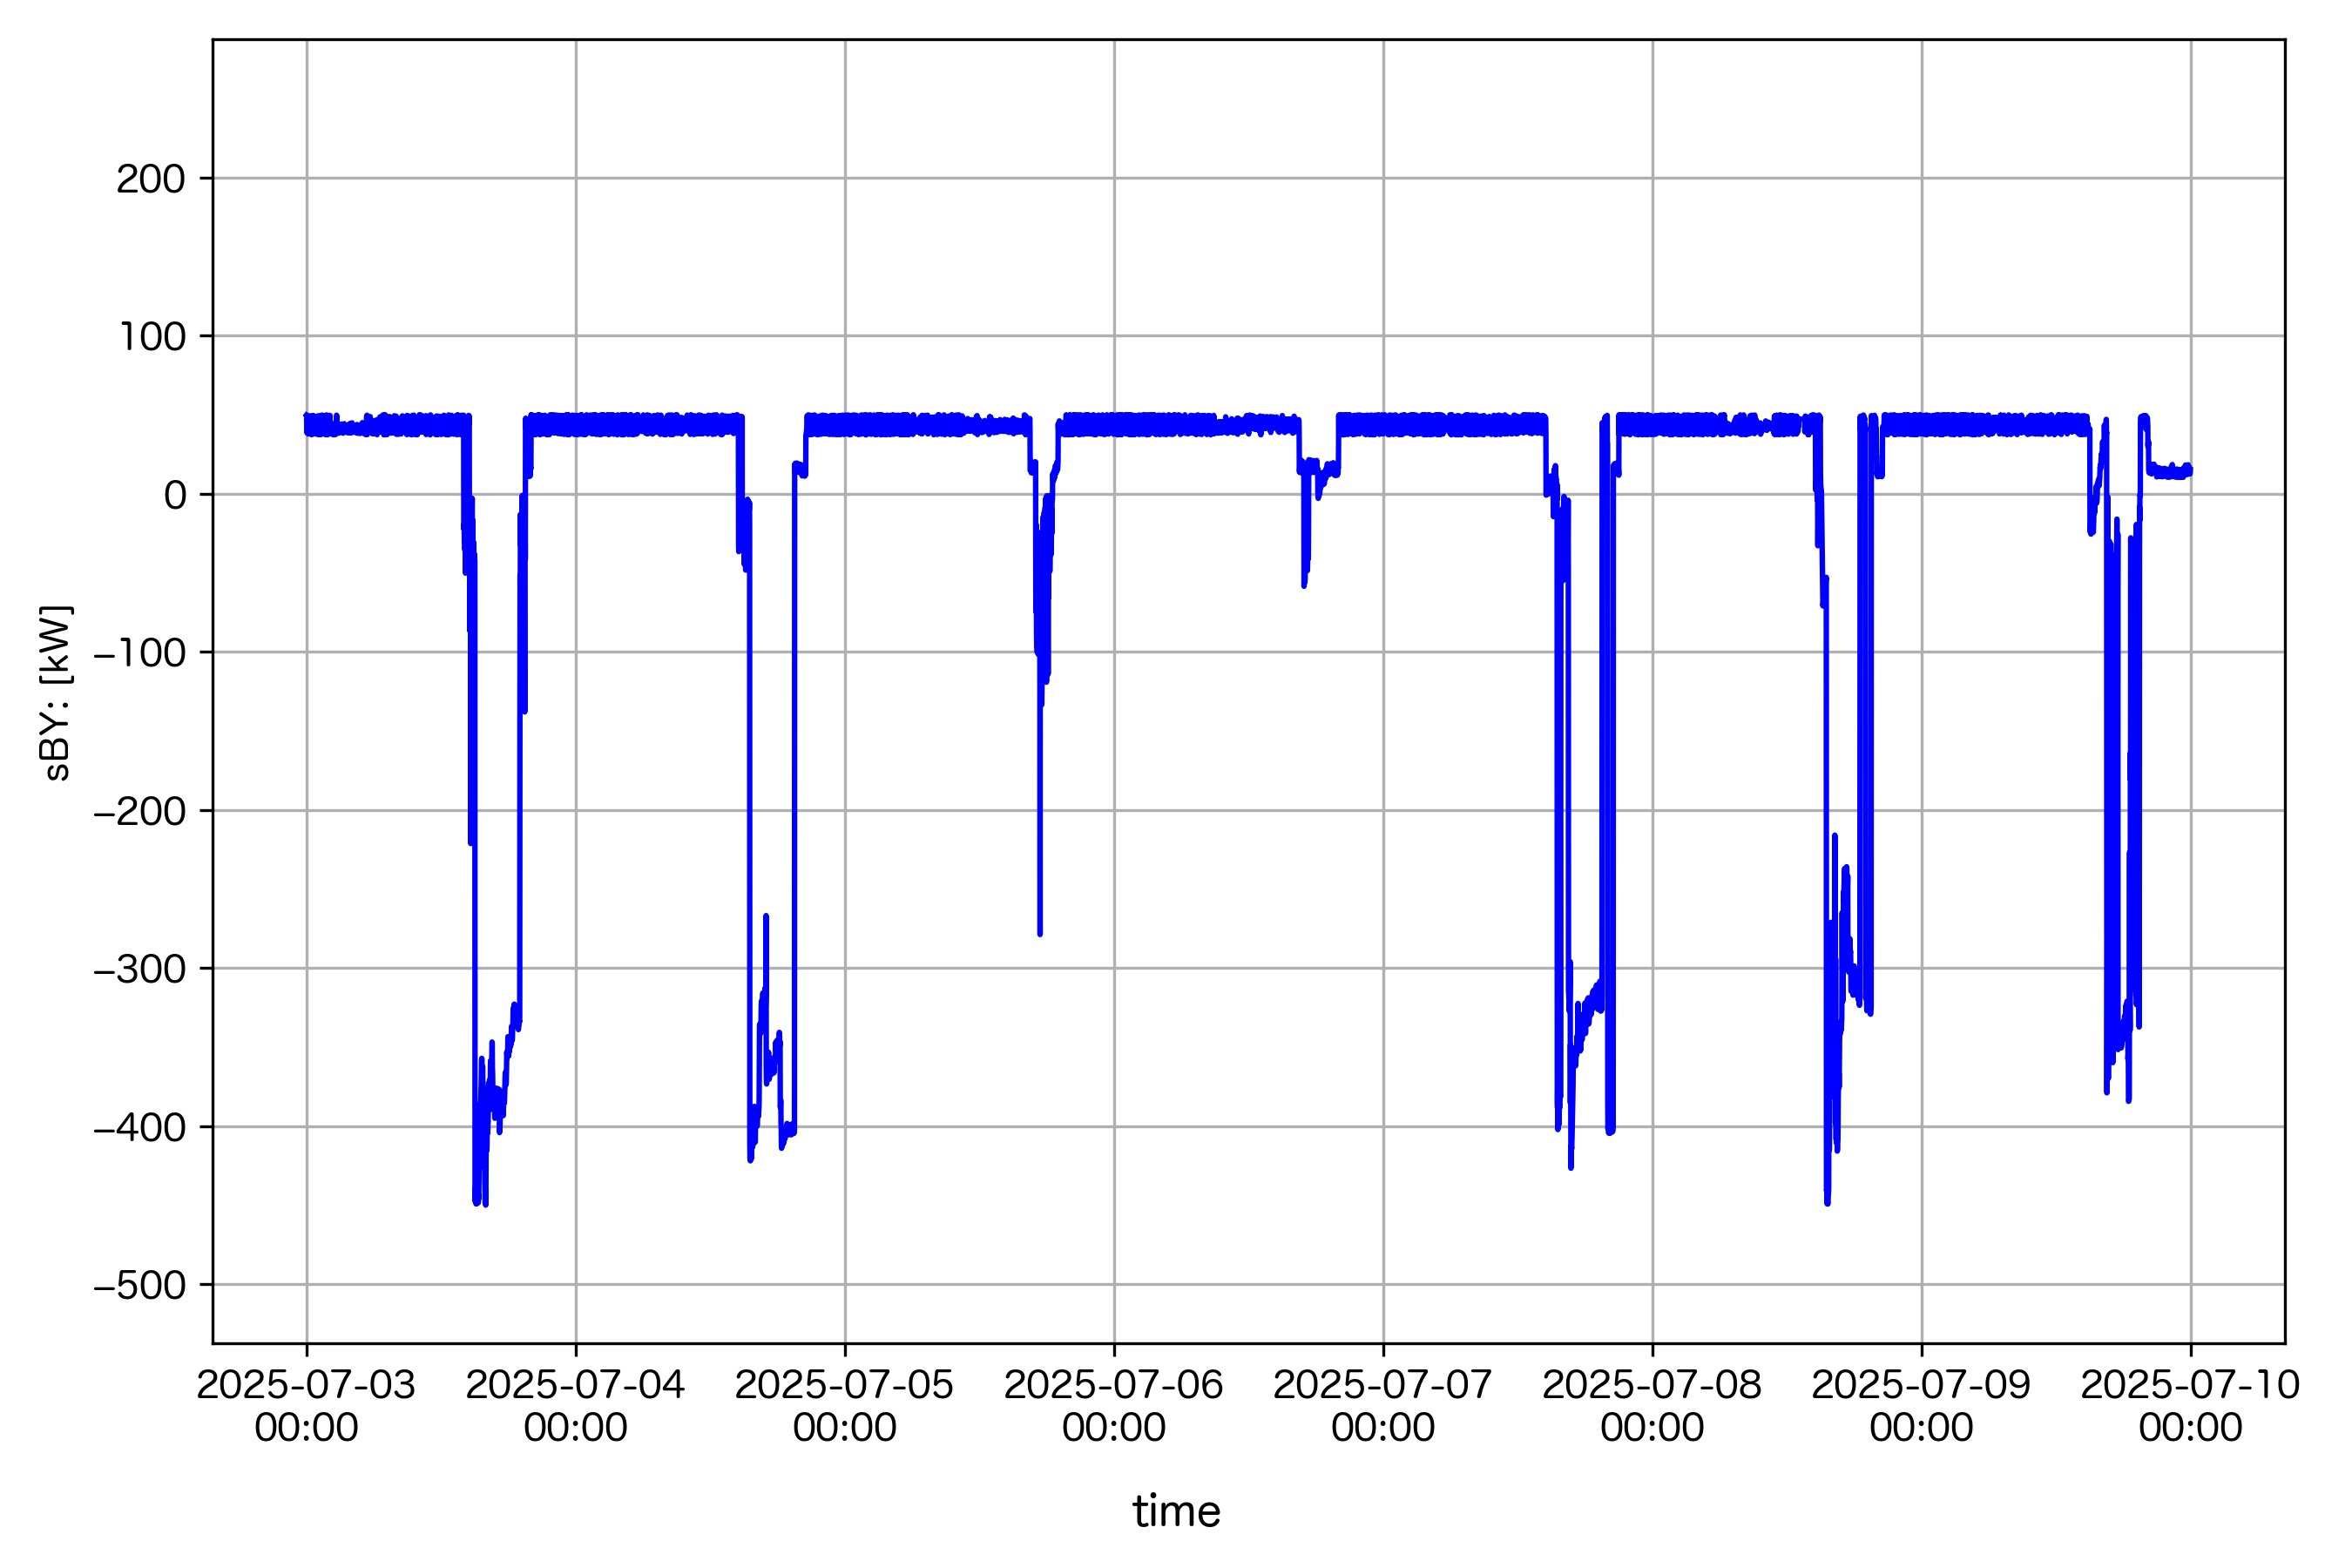
\includegraphics[width=120mm]{../figure/dp/sBY.png}
 	\caption{Grid Power Purchase}
 	\label{fig:dp_sBY_sSL}
\end{figure}

\begin{figure}[h]
	\centering
 	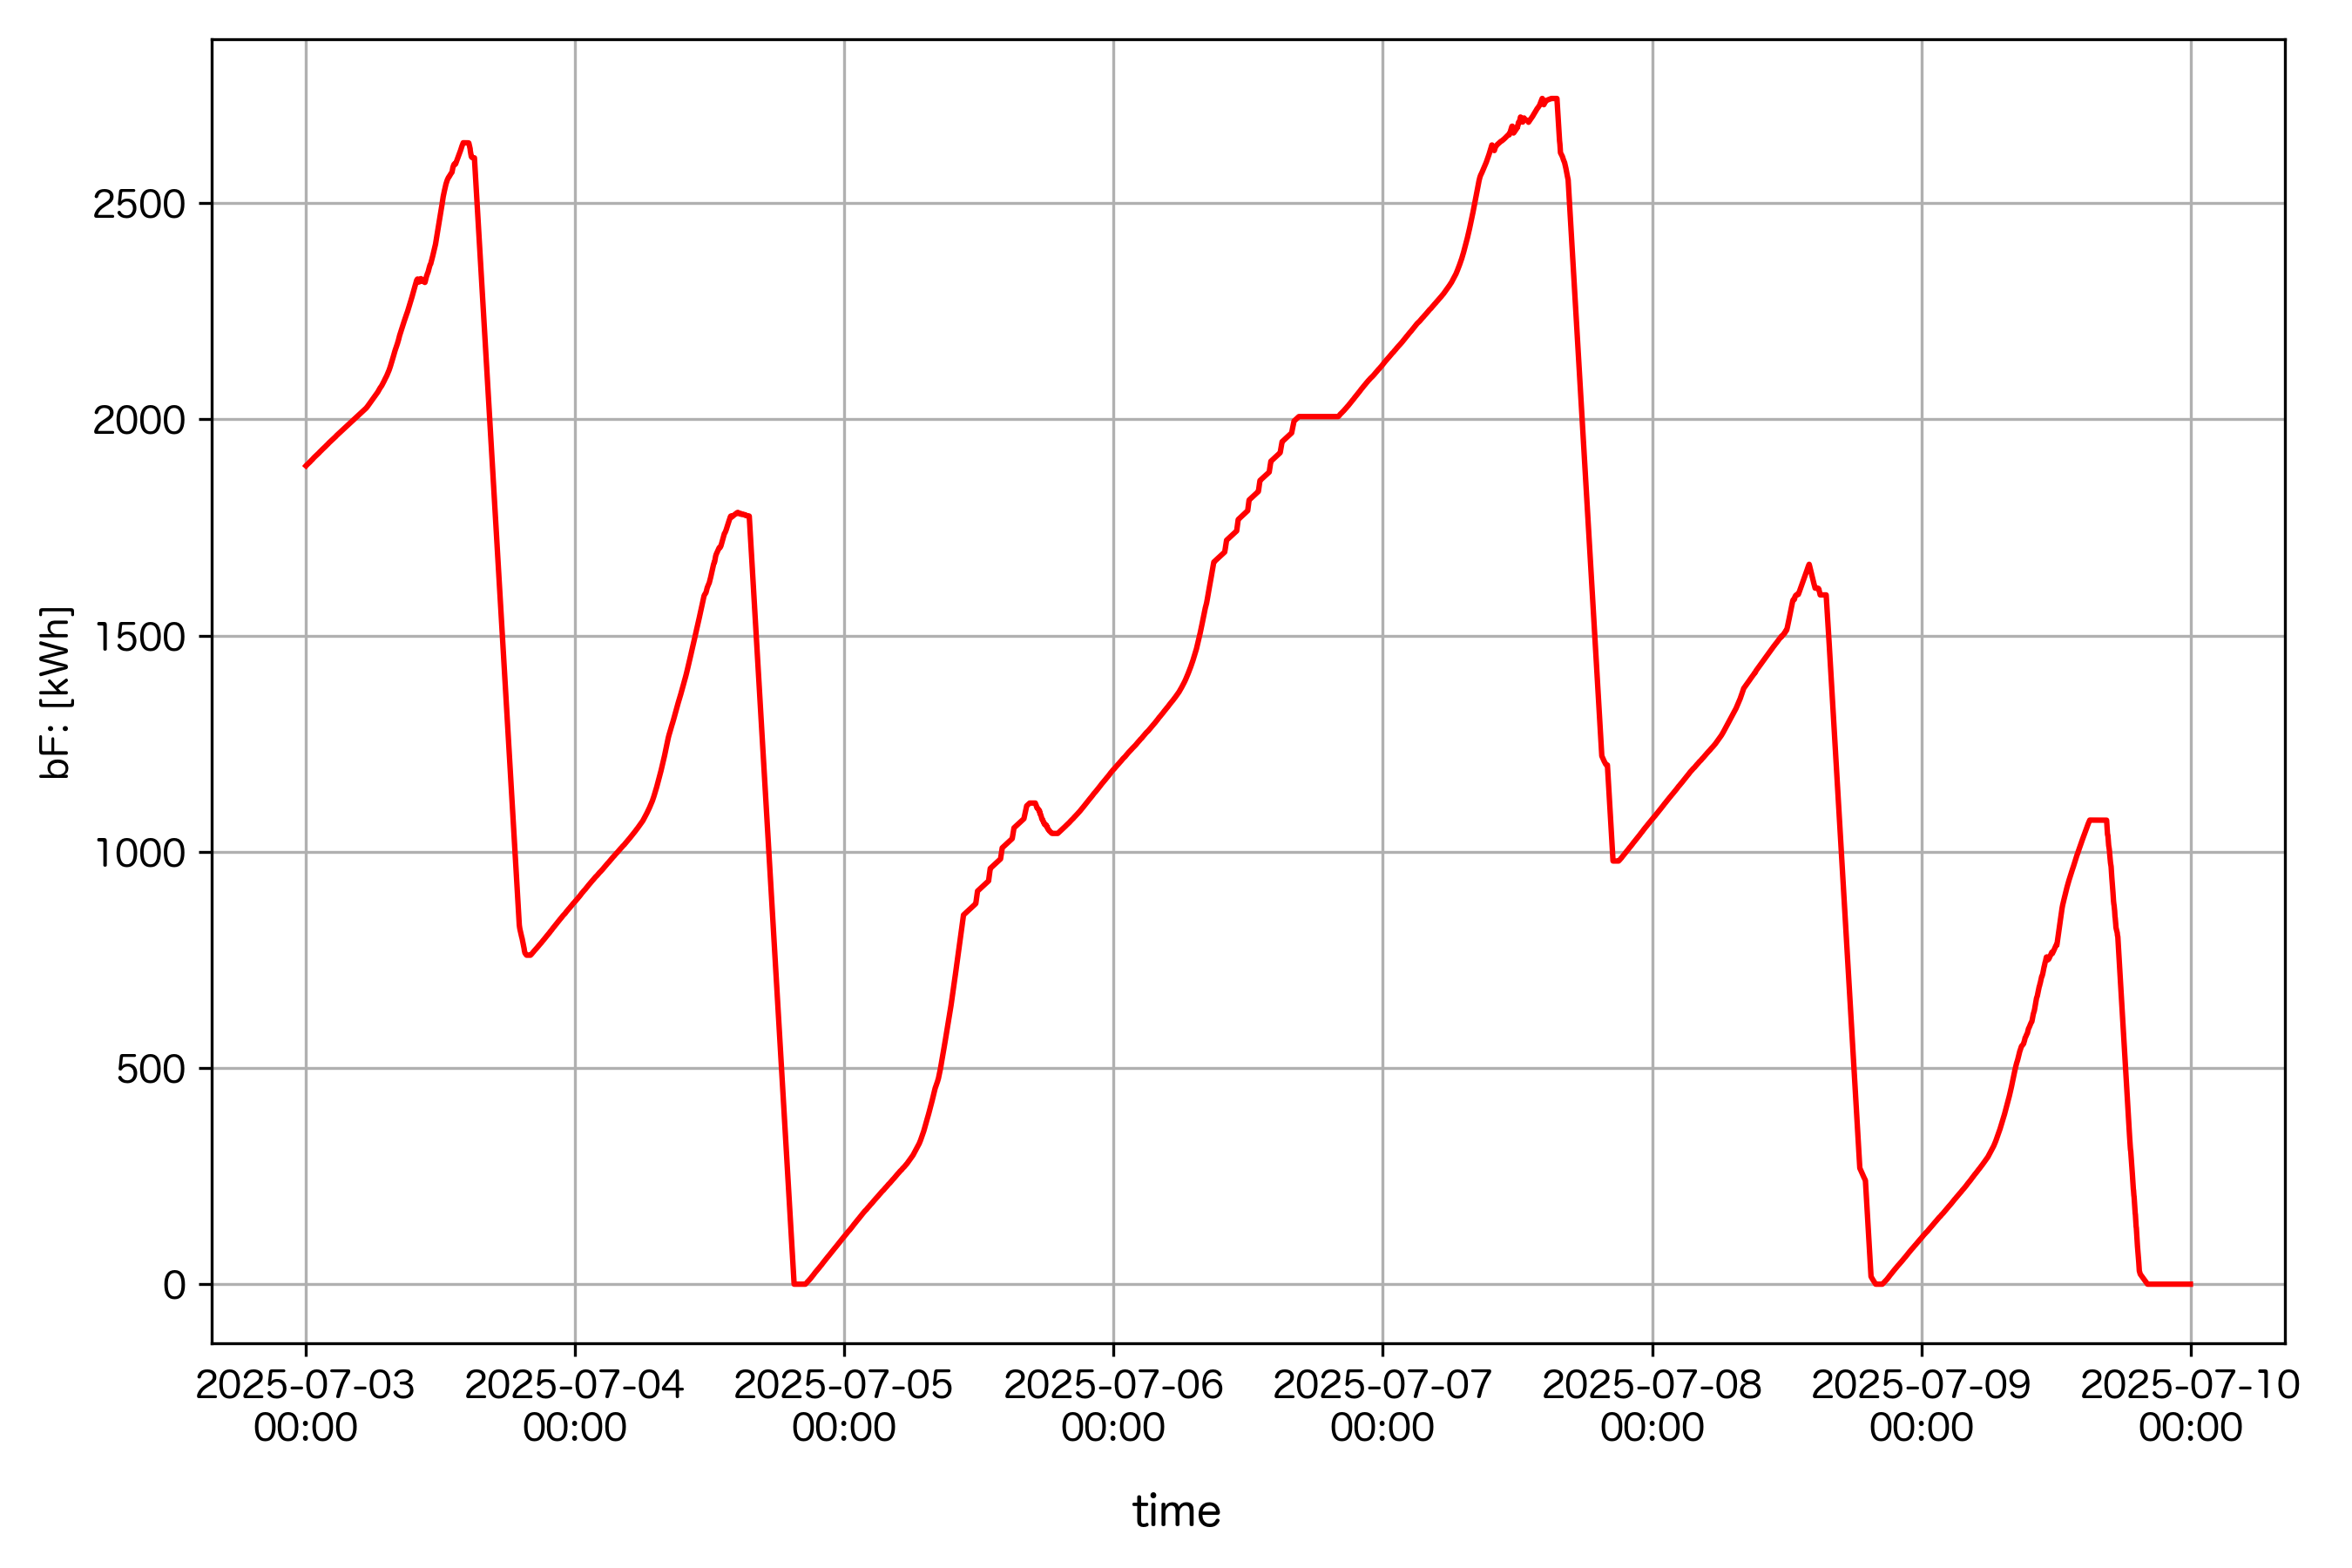
\includegraphics[width=120mm]{../figure/dp/bF.png}
 	\caption{Battery State of Charge}
 	\label{fig:dp_bF}
\end{figure}

\section{線形計画モデルと動的計画モデルの目的関数値の比較}
本節では，両モデルによって導出された最適目的関数値を比較し，動的計画モデルの解の質について評価を行う．
また，動的計画モデルにおける蓄電池残量の分割数$B$が解の精度に与える影響についても検証する．
表\ref{table:objective_comparison}に，各モデルにおける最適目的関数値を示す．
ここで，動的計画モデルについては，分割数$B$を本例題と同様である10080と，本例題の2倍とした20160，および本例題の1/2倍とした5040の
3つのケースにおける結果を示した．
なお，目的関数値は正味の支出を表しており負の値は利益，すなわち，売電収益が買電コストを上回った状態を意味する．

\begin{table}[htbp]
  \centering
  \caption{Comparison of Optimal Objective Function Values}
  \label{table:objective_comparison}
  \begin{tabular}{lcc}
    \hline
    Model & Objective Value\\
    \hline \hline
    Linear Programming & -101134.17\\
    Dynamic Programming(B=5040)& -86401.59\\
    Dynamic Programming(B=10080)& -93021.65\\
    Dynamic Programming(B=20160)& -96462.09\\
    \hline
  \end{tabular}
\end{table}

線形計画モデルは，変数が連続値をとるため離散化誤差を含まず，かつ制約条件においても「任意の連続する30分間の区間について，
商用電力系統からの総買電力を 50 kW以下に制限すること」という本来の制約を適用できている．
したがって，線形計画モデルによる解は，本問題における理論的な最大利益であるベンチマークとみなすことができる．
そこで，線形計画モデルの目的関数値を基準とした際の，動的計画モデルの相対誤差$E^{\rm gap}$を式\eqref{eq:gap}により定義し，評価を行う．

\begin{equation}
E^{\rm gap} = \frac{| J_{\rm DP}^*- J_{\rm LP}^* |}{| J_{\rm LP}^* |} \times 100
\label{eq:gap}
\end{equation}
ここで，$J_{\rm LP}^* $，$J_{\rm DP}^*$はそれぞれ線形計画モデルと動的計画モデルの最適目的関数値を表す．
式\eqref{eq:gap}に基づいて，各分割数$B$における相対誤差を計算した結果について検討する．
まず，本例題の設定である分割数 $B=10080$ の場合，相対誤差は約$8.02 \%$ となった．
これは線形計画モデルによる理論的な最大利益の約92\%を確保できていることを意味する．次に，離散化の粒度が解の精度に与える影響を確認するために，分割数$B$を変更した場合の結果を比較する．
分割数$B$を本例題の2倍である20160に設定し，状態空間の密度を高めた場合，目的関数値は-96462.09となり，相対誤差は$4.62 \%$ まで改善した．
一方で，分割数$B$を本例題の1/2倍である5040とし，状態空間を粗くした場合，目的関数値は-86401.59となり，相対誤差は$14.57 \%$ まで拡大した．

この結果から，分割数$B$を大きくし状態空間を密にするほど，動的計画モデルの解が線形計画モデルによる厳密解に漸近していくといえる．

\section{線形計画モデルと動的計画法モデルの計算時間の比較}
本節では，線形計画法および動的計画法を用いた際の計算時間を比較し，
各手法の特性について考察する．実験に使用した環境を表\ref{table:environment}に示す．
本検証では，前述のケース2を対象として，プログラムの開始から最適解の導出に至るまでの実行時間を計測した．
計算時間についてはプログラムの開始から最適解を導出するまでの時間である実行時間を計測した．
実行時間は，外部入力に伴う時間であるI/O時間と，ソルバーによる最適化を行う時間であるCPU時間に分類し，
各条件で5回計測した平均値を採用している．期の数$K$を5040，10080，15120，20160（それぞれの値は1期あたり1分とした場合，0.5週間，1週間，1.5週間，2週間に相当する）と，蓄電池の段階数$B$を6855，13710，27420(それぞれの値は蓄電池の最大容量を2742 kWhとした場合，蓄電池の刻み幅が0.4 kWh，0.2 kWh，0.1kWhである状態に相当する)と変化させながら線形計画法と動的計画法のそれぞれについて計算時間を求めたものを表\ref{table:time_lp}，表\ref{table:time_dp}に示す．

\subsection{期の数に関する考察}
まずは，期の数$K$が計算時間に与える影響を考察する．表\ref{table:time_lp}より，本問題に対して線形計画法を用いた場合，CPU時間はおおよそ$K$に比例，あるいはそれ以上の次数で増加していることがわかる．ところで，求解アルゴリズムの内ではシンプレックス法が用いられているが，シンプレックス法の時間的計算量について，Dantzigらによると典型的な反復回数は制約条件の数に比例して増大し(その比例係数は3/2〜3程度)，変数の数に関してはきわめてゆっくりと増大するといった理論的解釈が提案されている\cite{h}\cite{l}．しかしながら，最悪の場合の反復回数は問題の規模に対して指数関数的に増加することも知られている．
指数関数的に反復回数が増加する線形計画問題の例として，KleeとMintyは
\begin{equation}
	\text{max} \quad \sum_{j=1}^n 10^{n-j}x_j
	\label{eq:Klee_Minty_max}
\end{equation}
\begin{equation}
	\text{sub. to} \quad 2\sum_{j=1}^{i-j} 10^{i-j}x_j + x_i \leq 100^{i-1} \quad (i=1,\ldots, n)
	\label{eq:Klee_Minty_sub1}
\end{equation}
\begin{equation}
	 \quad  x_{j} \geq 0 \quad (j=1,\ldots, n)
	\label{eq:Klee_Minty_sub2}
\end{equation}
を解く過程でシンプレックス法の反復回数が$2^n-1$回になることを示している\cite{k}．
ただし，このようなケースは「病的」ともいわれるほどに特殊なケースであり，現実的な問題のほとんど全てに対してDantzigらによる反復回数の見積もりが有効である\cite{h}．
本実験結果においても，CPU時間がおよそ $K$ に比例して増加する挙動が確認された．

一方，動的計画法を用いた結果を示す表\ref{table:time_dp}においても，CPU時間は $K$ に比例して増加している．本モデルに対する動的計画法の時間的計算量は\\
 $O(B\{ \frac{(B-1)(\Delta s_k^{\mathrm{Max}}(s_{k-1}) - \Delta s_k^{\mathrm{Min}}(s_{k-1}) )}{\overline{b}} +1\} K)$ であり，本実験結果においてもCPU時間がおよそ$K$に
比例して増加する挙動が確認された．$K$ の増加に対する影響に注目すると，ある規模までは線形計画法が高速であるが，ステップ数がさらに増大する場合には，
計算量の増加量が小さい，動的計画法が有利になるといえる．

\subsection{蓄電池の残量の分割数に関する考察}
次に，蓄電池の残量の分割数$B$ が計算時間に与える影響を考察する．表\ref{table:time_dp}より，$B$ を2倍に拡張すると，CPU時間はおおよそ4倍に増大していることが確認できる．これは前述した時間的計算量における $B$ の2乗の寄与を裏付けるものであり，
$B$の値が比較的小さい条件下では動的計画法が線形計画法を上回る速度で最適解を導出可能である．
\begin{table}[htbp]
  \centering
  \caption{System specifications}
  \label{table:environment}
  \begin{tabular}{ll}
    \hline
    Item & Specifications \\
    \hline \hline
    CPU & Intel Core i5 1.4 GHz Quad-Core \\
    RAM & 16 GB (2133 MHz) \\
    OS & macOS Ventura 13.7.8 \\
    Programming Language & Python 3.9.12 \\
    Libraries (Common) & Pandas, NumPy, Matplotlib, os, unicodedata \\ 
    Library (LP) & PySCIPOpt \\
    Library (DP) & Numba \\
    \hline
  \end{tabular}
\end{table}

\begin{table}[htbp]
  \centering
  \caption{computation time (linear programming)}
  \label{table:time_lp}
  \begin{tabular}{ccc}
    \hline
    $K$ & I/O Time [s] & CPU Time [s] \\ 
    \hline \hline
    5040  & 2.59  & 7.96  \\
    10080 & 4.15  & 25.25 \\
    15120 & 7.97  & 44.40 \\
    20160 & 10.14 & 70.60 \\
    \hline
  \end{tabular}
\end{table}

\begin{table}[htbp]
  \centering
  \caption{computation time (dynamic programming)}
  \label{table:time_dp}
  \begin{tabular}{cccc}
    \hline
    $K$ & $B$ & I/O Time [s] & CPU Time [s] \\
    \hline \hline
    5040  & \multirow{4}{*}{6,855}  & 2.50 & 5.65  \\
    10080 &                         & 4.29 & 10.83 \\
    15120 &                         & 6.48 & 14.15 \\
    20160 &                         & 8.86 & 18.95 \\
    \hline
    5040  & \multirow{4}{*}{13,710} & 2.67 & 18.43 \\
    10080 &                         & 4.42 & 34.68 \\
    15120 &                         & 6.92 & 49.33 \\
    20160 &                         & 9.00 & 67.57 \\
    \hline
    5040  & \multirow{4}{*}{27,420} & 2.60 & 62.64  \\
    10080 &                         & 4.13 & 125.03 \\
    15120 &                         & 6.79 & 180.09 \\
    20160 &                         & 8.90 & 245.12 \\
    \hline
  \end{tabular}
\end{table}

\section{線形計画モデルと動的計画モデルの特徴のまとめ}
本節では，本章における計算結果および考察に基づき，電力運用最適化問題における線形計画モデルと動的計画モデルの特性を総括する．

線形計画モデルの利点は，解の厳密性と複数の期にまたがる制約条件に対する柔軟性にある．このモデルでは変数を連続値として扱うため離散化誤差が発生せず，
本計算例で示した通り理論的な最適解を得ることができる．また，30分間の平均電力を制限するといった期を跨ぐ制約条件が存在した場合においても，
計算時間を大きく増やすことなく求解が可能である．対して欠点として，期の数が多い場合，計算時間が大きく増加するという点がある．

一方で動的計画モデルの利点は，計算時間のスケーラビリティにある．計算時間は期の数に対して厳密に線形に増加するため，
長期間の運用計画を策定する場合でも所要時間の見積もりが容易である．
しかし，離散化誤差と制約条件の扱いに課題が残る．解の精度を向上させるために分割数を増やすと計算時間が大幅に増大するため，
精度と計算時間の間に強いトレードオフが発生する．加えて，期間を跨ぐ制約条件を導入する場合，状態空間の拡張が必要となり計算量が爆発的に増加するため，
より厳しい制約への置き換えを余儀なくされる場合がある．これが探索空間を狭め，解の質を低下させる要因となる．

結論として，高い精度や複数の期にまたがる複雑な制約条件への対応が求められる場合には線形計画モデルが適しており，
長期間のシミュレーションにおいて計算時間の見通しを重視するといったように多くの期を必要とする場合については動的計画モデルが適しているといえる．




